\PassOptionsToPackage{unicode=true}{hyperref} % options for packages loaded elsewhere
\PassOptionsToPackage{hyphens}{url}
%
\documentclass[a4paperpaper,openright]{book}
\usepackage{lmodern}
\usepackage{amssymb,amsmath}
\usepackage{ifxetex,ifluatex}
\usepackage{fixltx2e} % provides \textsubscript
\ifnum 0\ifxetex 1\fi\ifluatex 1\fi=0 % if pdftex
  \usepackage[T1]{fontenc}
  \usepackage[utf8]{inputenc}
  \usepackage{textcomp} % provides euro and other symbols
\else % if luatex or xelatex
  \usepackage{unicode-math}
  \defaultfontfeatures{Ligatures=TeX,Scale=MatchLowercase}
\fi
% use upquote if available, for straight quotes in verbatim environments
\IfFileExists{upquote.sty}{\usepackage{upquote}}{}
% use microtype if available
\IfFileExists{microtype.sty}{%
\usepackage[]{microtype}
\UseMicrotypeSet[protrusion]{basicmath} % disable protrusion for tt fonts
}{}
\IfFileExists{parskip.sty}{%
\usepackage{parskip}
}{% else
\setlength{\parindent}{0pt}
\setlength{\parskip}{6pt plus 2pt minus 1pt}
}
\usepackage{hyperref}
\hypersetup{
            pdfborder={0 0 0},
            breaklinks=true}
\urlstyle{same}  % don't use monospace font for urls
\usepackage{color}
\usepackage{fancyvrb}
\newcommand{\VerbBar}{|}
\newcommand{\VERB}{\Verb[commandchars=\\\{\}]}
\DefineVerbatimEnvironment{Highlighting}{Verbatim}{commandchars=\\\{\}}
% Add ',fontsize=\small' for more characters per line
\newenvironment{Shaded}{}{}
\newcommand{\AlertTok}[1]{\textcolor[rgb]{1.00,0.00,0.00}{\textbf{#1}}}
\newcommand{\AnnotationTok}[1]{\textcolor[rgb]{0.38,0.63,0.69}{\textbf{\textit{#1}}}}
\newcommand{\AttributeTok}[1]{\textcolor[rgb]{0.49,0.56,0.16}{#1}}
\newcommand{\BaseNTok}[1]{\textcolor[rgb]{0.25,0.63,0.44}{#1}}
\newcommand{\BuiltInTok}[1]{#1}
\newcommand{\CharTok}[1]{\textcolor[rgb]{0.25,0.44,0.63}{#1}}
\newcommand{\CommentTok}[1]{\textcolor[rgb]{0.38,0.63,0.69}{\textit{#1}}}
\newcommand{\CommentVarTok}[1]{\textcolor[rgb]{0.38,0.63,0.69}{\textbf{\textit{#1}}}}
\newcommand{\ConstantTok}[1]{\textcolor[rgb]{0.53,0.00,0.00}{#1}}
\newcommand{\ControlFlowTok}[1]{\textcolor[rgb]{0.00,0.44,0.13}{\textbf{#1}}}
\newcommand{\DataTypeTok}[1]{\textcolor[rgb]{0.56,0.13,0.00}{#1}}
\newcommand{\DecValTok}[1]{\textcolor[rgb]{0.25,0.63,0.44}{#1}}
\newcommand{\DocumentationTok}[1]{\textcolor[rgb]{0.73,0.13,0.13}{\textit{#1}}}
\newcommand{\ErrorTok}[1]{\textcolor[rgb]{1.00,0.00,0.00}{\textbf{#1}}}
\newcommand{\ExtensionTok}[1]{#1}
\newcommand{\FloatTok}[1]{\textcolor[rgb]{0.25,0.63,0.44}{#1}}
\newcommand{\FunctionTok}[1]{\textcolor[rgb]{0.02,0.16,0.49}{#1}}
\newcommand{\ImportTok}[1]{#1}
\newcommand{\InformationTok}[1]{\textcolor[rgb]{0.38,0.63,0.69}{\textbf{\textit{#1}}}}
\newcommand{\KeywordTok}[1]{\textcolor[rgb]{0.00,0.44,0.13}{\textbf{#1}}}
\newcommand{\NormalTok}[1]{#1}
\newcommand{\OperatorTok}[1]{\textcolor[rgb]{0.40,0.40,0.40}{#1}}
\newcommand{\OtherTok}[1]{\textcolor[rgb]{0.00,0.44,0.13}{#1}}
\newcommand{\PreprocessorTok}[1]{\textcolor[rgb]{0.74,0.48,0.00}{#1}}
\newcommand{\RegionMarkerTok}[1]{#1}
\newcommand{\SpecialCharTok}[1]{\textcolor[rgb]{0.25,0.44,0.63}{#1}}
\newcommand{\SpecialStringTok}[1]{\textcolor[rgb]{0.73,0.40,0.53}{#1}}
\newcommand{\StringTok}[1]{\textcolor[rgb]{0.25,0.44,0.63}{#1}}
\newcommand{\VariableTok}[1]{\textcolor[rgb]{0.10,0.09,0.49}{#1}}
\newcommand{\VerbatimStringTok}[1]{\textcolor[rgb]{0.25,0.44,0.63}{#1}}
\newcommand{\WarningTok}[1]{\textcolor[rgb]{0.38,0.63,0.69}{\textbf{\textit{#1}}}}
\usepackage{graphicx,grffile}
\makeatletter
\def\maxwidth{\ifdim\Gin@nat@width>\linewidth\linewidth\else\Gin@nat@width\fi}
\def\maxheight{\ifdim\Gin@nat@height>\textheight\textheight\else\Gin@nat@height\fi}
\makeatother
% Scale images if necessary, so that they will not overflow the page
% margins by default, and it is still possible to overwrite the defaults
% using explicit options in \includegraphics[width, height, ...]{}
\setkeys{Gin}{width=\maxwidth,height=\maxheight,keepaspectratio}
\setlength{\emergencystretch}{3em}  % prevent overfull lines
\providecommand{\tightlist}{%
  \setlength{\itemsep}{0pt}\setlength{\parskip}{0pt}}
\setcounter{secnumdepth}{0}
% Redefines (sub)paragraphs to behave more like sections
\ifx\paragraph\undefined\else
\let\oldparagraph\paragraph
\renewcommand{\paragraph}[1]{\oldparagraph{#1}\mbox{}}
\fi
\ifx\subparagraph\undefined\else
\let\oldsubparagraph\subparagraph
\renewcommand{\subparagraph}[1]{\oldsubparagraph{#1}\mbox{}}
\fi

% set default figure placement to htbp
\makeatletter
\def\fps@figure{htbp}
\makeatother

% Table of contents formatting
\renewcommand{\contentsname}{Table of Contents}
\setcounter{tocdepth}{3}

\setcounter{secnumdepth}{4}


% \renewcommand\thesection{\Roman{section}}

 
% Headers and page numbering 
\usepackage{fancyhdr}

\fancyhead{}
\fancyhead[R]{\leftmark}
\renewcommand{\headrulewidth}{0.4pt}

\fancyfoot[R]{\thepage}
\fancyfoot[C]{}
\fancyfoot[L]{\textit{An Introduction to Symfony 6 \copyright Matt Smith 2022}}
\renewcommand{\footrulewidth}{0.4pt}

\pagestyle{fancy}

% Fonts and typesetting
\setsansfont{Verdana}

% Set figure legends and captions to be smaller sized sans serif font
\usepackage[font={footnotesize,sf}]{caption}

\usepackage{siunitx}

% Adjust spacing between lines to 1.5
\usepackage{setspace}
\onehalfspacing
\raggedbottom

% Set margins
\usepackage[top=1.25in,bottom=1.25in]{geometry}

% Chapter styling
\usepackage[grey]{quotchap}
\makeatletter
\renewcommand*{\chapnumfont}{%
  \usefont{T1}{\@defaultcnfont}{b}{n}\fontsize{80}{100}\selectfont% Default: 100/130
  \color{chaptergrey}%
}
\makeatother

% Set colour of links to black so that they don't show up when printed
\usepackage{hyperref}
\hypersetup{colorlinks=true, linkcolor=black}

% Tables
\usepackage{booktabs}
\usepackage{threeparttable}
\usepackage{array}
\newcolumntype{x}[1]{%
>{\centering\arraybackslash}m{#1}}%

% Allow for long captions and float captions on opposite page of figures 
\usepackage[rightFloats, CaptionBefore]{fltpage}

% Don't let floats cross subsections
\usepackage[section,subsection]{extraplaceins}

\date{}

\begin{document}

\begin{titlepage}
    \begin{center}
    
        \vspace*{1cm}
        

       \large{ \textbf{ \uppercase{An Introduction to Symfony 6}\\(for people that already know OO-PHP and some MVC stuff)}}
        
        \vspace{1.5cm}

        by\\
        \textbf{
        Matt Smith, Ph.D.\\https://github.com/dr-matt-smith
        }

       

        
        
        \vfill
  
            \copyright ~ 2022

     \end{center}
    \thispagestyle{empty}
\end{titlepage}

\newpage
\thispagestyle{empty}
\mbox{}

\frontmatter

\chapter{Acknowledgements}

Thanks to Ryan Weaver, for suggesting I update things to Symfony 6 in
2022 :-)

Thanks to the PHP and Symfony open-source international communities.

\tableofcontents

\mainmatter

\part{Security and Authentication}

\hypertarget{quickstart-symfony-security}{%
\chapter{Quickstart Symfony
security}\label{quickstart-symfony-security}}

\hypertarget{learn-about-symfony-security}{%
\section{Learn about Symfony
security}\label{learn-about-symfony-security}}

There are several key Symfony reference pages to read when starting with
security. These include:

\begin{itemize}
\item
  Introduction to security

  \begin{itemize}
  \tightlist
  \item
    \url{https://symfony.com/doc/current/security.html}
  \end{itemize}
\item
  How to build a traditional login form

  \begin{itemize}
  \tightlist
  \item
    \url{https://symfony.com/doc/current/security/form_login_setup.html}
  \end{itemize}
\item
  Using CSRF protection

  \begin{itemize}
  \tightlist
  \item
    \url{https://symfony.com/doc/current/security/csrf.html}
  \end{itemize}
\end{itemize}

\hypertarget{new-project-with-open-and-secured-routes-project-security01}{%
\section{\texorpdfstring{New project with open and secured routes
(project
\texttt{security01})}{New project with open and secured routes (project security01)}}\label{new-project-with-open-and-secured-routes-project-security01}}

We are going to quickly create a 2-page website, with an open home page
(url \texttt{/}) and a secured admin page (at url \texttt{/admin}).

\hypertarget{create-new-project-and-add-the-security-bundle-library}{%
\section{Create new project and add the security bundle
library}\label{create-new-project-and-add-the-security-bundle-library}}

Create a new project:

\begin{Shaded}
\begin{Highlighting}[]
  \ExtensionTok{symfony}\NormalTok{ new --webapp security01}
\end{Highlighting}
\end{Shaded}

Add the fixtures bundle (we'll need this later):

\begin{Shaded}
\begin{Highlighting}[]
    \ExtensionTok{composer}\NormalTok{ require orm-fixtures}
\end{Highlighting}
\end{Shaded}

\hypertarget{make-a-default-controller}{%
\section{Make a Default controller}\label{make-a-default-controller}}

Let's make a Default controller
\texttt{/src/Controller/DefaultController.php}:

\begin{Shaded}
\begin{Highlighting}[]
    \ExtensionTok{symfony}\NormalTok{ console make:controller Default}
\end{Highlighting}
\end{Shaded}

Edit the route URL to be simply \texttt{/}, and the internal name to be
\texttt{homepage}. Also simplify the body of the method, so we can
clearly see that we are passing an empty array of arguments to template
\texttt{default/index.html.twig}:

\begin{Shaded}
\begin{Highlighting}[]
    \CommentTok{#[Route('/', name: 'homepage')]}
    \KeywordTok{public} \KeywordTok{function}\NormalTok{ index}\OtherTok{()}\NormalTok{: Response}
\NormalTok{    \{}
        \KeywordTok{$template}\NormalTok{ = }\StringTok{'default/index.html.twig'}\OtherTok{;}
        \KeywordTok{$args}\NormalTok{ = }\OtherTok{[];}
        \KeywordTok{return} \KeywordTok{$this}\NormalTok{->render}\OtherTok{(}\KeywordTok{$template}\OtherTok{,} \KeywordTok{$args}\OtherTok{);}
\NormalTok{    \}}
\end{Highlighting}
\end{Shaded}

Change the template \texttt{/templates/default/index.html.twig} to be
something like:

\begin{verbatim}
    

    
        welcome to the home page
    
\end{verbatim}

This will be accessible to everyone.

Test the server, and if necessary, remove the \texttt{encore\_entry\_}
lines inside the \texttt{stylesheets} and \texttt{javascripts} blocks in
the base template (\texttt{/templates/base.html.twig}).

\hypertarget{make-an-un-secured-admin-controller}{%
\section{Make an un-secured Admin
controller}\label{make-an-un-secured-admin-controller}}

Let's make a Admin controller:

\begin{Shaded}
\begin{Highlighting}[]
\NormalTok{    $ }\ExtensionTok{symfony}\NormalTok{ console make:controller Admin}
\end{Highlighting}
\end{Shaded}

Change the default (index) admin template to be something like the
following - a secret code we can only see if logged in.

File: \texttt{/templates/admin/index.html.twig}:

\begin{verbatim}
    

    
        <h1>Admin home</h1>

        here is the secret code to the safe:
        007123
    
\end{verbatim}

That's it!

Run the web sever:

\begin{itemize}
\item
  visiting the Default page at \texttt{/} is fine, even though we have
  not logged in ag all
\item
  visiting the Admin page at \texttt{/admin} is fine too (for now),
  since we haven't added any security to this controller/method yet
\end{itemize}

\hypertarget{secure-the-admin-controller-for-only-logged-in-users-with-role_admin}{%
\section{\texorpdfstring{Secure the Admin controller for only logged in
users with
\texttt{ROLE\_ADMIN}}{Secure the Admin controller for only logged in users with ROLE\_ADMIN}}\label{secure-the-admin-controller-for-only-logged-in-users-with-role_admin}}

Let's now make the admin home page only accessible to only to users
logged in with \texttt{ROLE\_ADMIN} security.

Edit the new \texttt{AdminController} in
\texttt{/src/Controller/AdminController.php}. Add a \texttt{use}
statement, to let us use the \texttt{\#{[}IsGranted{]}} attribute:

\begin{Shaded}
\begin{Highlighting}[]
    \KeywordTok{use}\NormalTok{ Sensio\textbackslash{}Bundle\textbackslash{}FrameworkExtraBundle\textbackslash{}Configuration\textbackslash{}IsGranted}\OtherTok{;}
\end{Highlighting}
\end{Shaded}

Now we'll restrict access to the index action of our Admin controller
using the \texttt{\#{[}IsGranted{]}} attribute. Symfony security expects
logged-in users to have one or more `roles', these are simple text
Strings in the form \texttt{ROLE\_xxxx}. The default is to have all
logged-in users having \texttt{ROLE\_USER}, and they can have additional
roles as well. So let's restrict our admin home page to only logged-in
users that have the authentication \texttt{ROLE\_ADMIN}:

\begin{Shaded}
\begin{Highlighting}[]
    \StringTok{...}
    \KeywordTok{use}\NormalTok{ Sensio\textbackslash{}Bundle\textbackslash{}FrameworkExtraBundle\textbackslash{}Configuration\textbackslash{}IsGranted}\OtherTok{;}

    \KeywordTok{class}\NormalTok{ AdminController }\KeywordTok{extends}\NormalTok{ AbstractController}
\NormalTok{    \{}
        \CommentTok{#[Route('/admin', name: 'app_admin')]}
        \CommentTok{#[IsGranted('ROLE_ADMIN')]}
        \KeywordTok{public} \KeywordTok{function}\NormalTok{ index}\OtherTok{()}\NormalTok{: Response}
\NormalTok{        \{}
            \KeywordTok{$template}\NormalTok{ = }\StringTok{'admin/index.html.twig'}\OtherTok{;}
            \KeywordTok{$args}\NormalTok{ = }\OtherTok{[];}
            \KeywordTok{return} \KeywordTok{$this}\NormalTok{->render}\OtherTok{(}\KeywordTok{$template}\OtherTok{,} \KeywordTok{$args}\OtherTok{);}
\NormalTok{        \}}
\NormalTok{    \}}
\end{Highlighting}
\end{Shaded}

NOTE: We can \textbf{make up} whatever roles are appropriate for our
application, e.g.:

\begin{Shaded}
\begin{Highlighting}[]
    \KeywordTok{ROLE_ADMIN}
    \KeywordTok{ROLE_STUDENT}
    \KeywordTok{ROLE_PRESIDENT}
    \KeywordTok{ROLE_TECHNICIAN}
    \StringTok{...}\NormalTok{ etc. }
\end{Highlighting}
\end{Shaded}

Now in the browser, visiting the the \texttt{/admin} page should result
in an HTTP 401 error (Unauthorized) due to insufficient authentication.
See Figure \ref{not_authorised}.

\begin{figure}
\centering
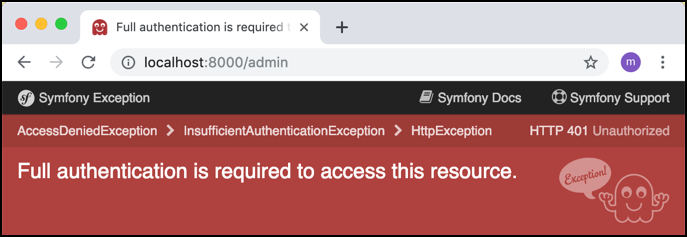
\includegraphics[width=0.75\textwidth,height=\textheight]{./tex2pdf.-40a8cafc9587c9a0/1f857b19819be887adb09dafdce063deff3936e3.png}
\caption{Screenshot of error attempting to visit \texttt{/admin}.
\label{not_authorised}}
\end{figure}

Of course, we now need to add a way to login and define different user
credentials etc\ldots{}

\hypertarget{core-features-about-symfony-security}{%
\section{Core features about Symfony
security}\label{core-features-about-symfony-security}}

There are several related features and files that need to be understood
when using the Symfony security system. These include:

\begin{itemize}
\tightlist
\item
  \textbf{firewalls}
\item
  \textbf{providers} and \textbf{encoders}
\item
  \textbf{route protection} (we met this with \texttt{\#{[}IsGranted{]}}
  controller method attribute above\ldots{})
\item
  user \textbf{roles} (we met this as part of \texttt{\#{[}IsGranted{]}}
  above \texttt{("ROLE\_ADMIN")} \ldots{})
\end{itemize}

Core to Symfony security are the \textbf{firewalls} defined in
\texttt{/config/packages/security.yml}. Symfony firewalls declare how
route patterns are protected (or not) by the security system. Here is
its default contents (less comments - lines starting with hash
\texttt{\#} character):

\begin{Shaded}
\begin{Highlighting}[]
    \FunctionTok{security:}
        \FunctionTok{enable_authenticator_manager:}\AttributeTok{ }\CharTok{true}

        \FunctionTok{password_hashers:}
            \FunctionTok{Symfony\textbackslash{}Component\textbackslash{}Security\textbackslash{}Core\textbackslash{}User\textbackslash{}PasswordAuthenticatedUserInterface:}\AttributeTok{ }\StringTok{'auto'}

        \FunctionTok{providers:}
            \FunctionTok{users_in_memory:}\AttributeTok{ }\KeywordTok{\{} \FunctionTok{memory:}\AttributeTok{ }\CharTok{null}\AttributeTok{ }\KeywordTok{\}}
        \FunctionTok{firewalls:}
            \FunctionTok{dev:}
                \FunctionTok{pattern:}\AttributeTok{ ^/(_(profiler|wdt)|css|images|js)/}
                \FunctionTok{security:}\AttributeTok{ }\CharTok{false}
            \FunctionTok{main:}
                \FunctionTok{lazy:}\AttributeTok{ }\CharTok{true}
                \FunctionTok{provider:}\AttributeTok{ users_in_memory}

        \FunctionTok{access_control:}
            \CommentTok{# - \{ path: ^/admin, roles: ROLE_ADMIN \}}
            \CommentTok{# - \{ path: ^/profile, roles: ROLE_USER \}}
\end{Highlighting}
\end{Shaded}

When no user has logged in, we can this looking at the user information
from the Symfony debug bar when visiting the default home page - see
Figure \ref{no_user}.

\begin{figure}
\centering
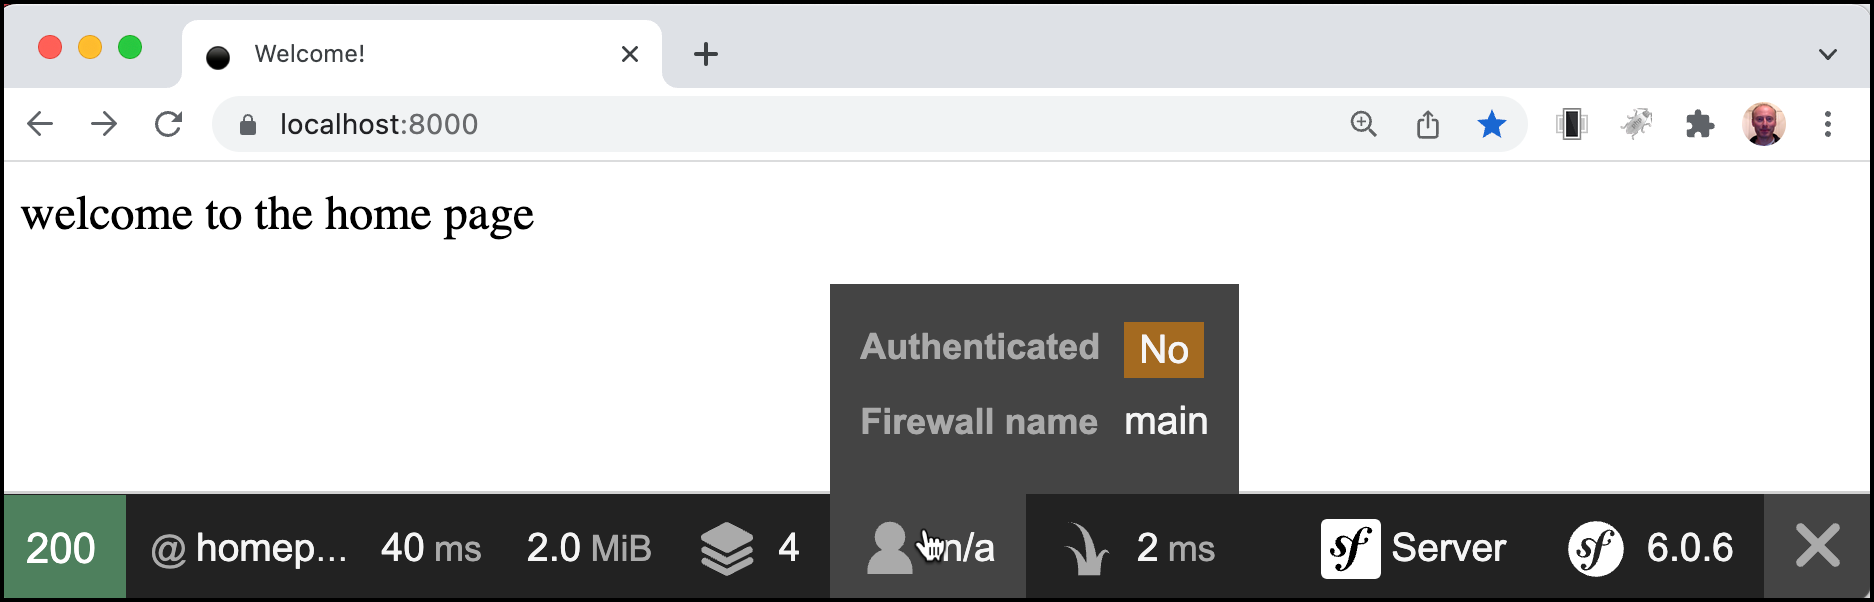
\includegraphics{./tex2pdf.-40a8cafc9587c9a0/776c1c4f283b0377be72c3956d13a16b81069fd4.png}
\caption{Symfony profiler showing no logged in authenticated user.
\label{no_user}}
\end{figure}

A Symfony \textbf{provider} is where the security system can access a
set of defined users of the web application. The default for a new
project is simply \texttt{in\_memory} - although non-trivial
applications have users in a database or from a separate API. We see
that the \texttt{main} firewall simply states that users are permitted
(at present) any request route pattern, and anonymous authenticated
users (i.e.~ones who have not logged in) are permitted.

The \texttt{dev} firewall allows Symfony development tools (like the
profiler) to work without any authentication required. Leave it in
\texttt{security.yml} and just ignore the \texttt{dev} firewall from
this point onwards.

\hypertarget{generating-the-special-user-entity-class}{%
\section{\texorpdfstring{Generating the special \texttt{User} Entity
class}{Generating the special User Entity class}}\label{generating-the-special-user-entity-class}}

Let's use the special \texttt{make:user} console command to create a
\texttt{User} entity class that meets the requirements of providing user
objects for the Symfony security system.

Enter the following at the command line, then just keep pressing
\texttt{\textless{}RETURN\textgreater{}} to accept all the defaults:

\begin{Shaded}
\begin{Highlighting}[]
\NormalTok{    $ }\ExtensionTok{symfony}\NormalTok{ console make:user}

     \ExtensionTok{The}\NormalTok{ name of the security user class (e.g. User) [}\ExtensionTok{User}\NormalTok{]:}
     \OperatorTok{>}          \ExtensionTok{//}\NormalTok{ press }\OperatorTok{<}\NormalTok{RETURN}\OperatorTok{>}\NormalTok{ to accept default}
    
     \ExtensionTok{Do}\NormalTok{ you want to store user data in the database (via Doctrine)}\ExtensionTok{?}\NormalTok{ (yes/no) [}\ExtensionTok{yes}\NormalTok{]:}
     \OperatorTok{>}          \ExtensionTok{//}\NormalTok{ press }\OperatorTok{<}\NormalTok{RETURN}\OperatorTok{>}\NormalTok{ to accept default}
    
     \ExtensionTok{Enter}\NormalTok{ a property name that will be the unique }\StringTok{"display"}\NormalTok{ name for the user (e.g. email, username, uuid) [}\ExtensionTok{email}\NormalTok{]:}
     \OperatorTok{>}          \ExtensionTok{//}\NormalTok{ press }\OperatorTok{<}\NormalTok{RETURN}\OperatorTok{>}\NormalTok{ to accept default}
    
     \ExtensionTok{Will}\NormalTok{ this app need to hash/check user passwords?}
     \ExtensionTok{Choose}\NormalTok{ No if passwords are not needed or will be checked/hashed by some other system (e.g. a single sign-on server)}\ExtensionTok{.}

     \ExtensionTok{Does}\NormalTok{ this app need to hash/check user passwords? (yes/no) [}\ExtensionTok{yes}\NormalTok{]:}
     \OperatorTok{>}          \ExtensionTok{//}\NormalTok{ press }\OperatorTok{<}\NormalTok{RETURN}\OperatorTok{>}\NormalTok{ to accept default}
    
     \ExtensionTok{created}\NormalTok{: src/Entity/User.php}
     \ExtensionTok{created}\NormalTok{: src/Repository/UserRepository.php}
     \ExtensionTok{updated}\NormalTok{: src/Entity/User.php}
     \ExtensionTok{updated}\NormalTok{: config/packages/security.yaml}
      \ExtensionTok{Success}\NormalTok{! }
\end{Highlighting}
\end{Shaded}

\hypertarget{review-the-changes-to-the-configpackagessecurity.yml-file}{%
\section{\texorpdfstring{Review the changes to the
\texttt{/config/packages/security.yml}
file}{Review the changes to the /config/packages/security.yml file}}\label{review-the-changes-to-the-configpackagessecurity.yml-file}}

If we look at \texttt{security.yml} it now begins as follows, taking
into account our new \texttt{User} class:

\begin{Shaded}
\begin{Highlighting}[]
    \FunctionTok{security:}
        \FunctionTok{enable_authenticator_manager:}\AttributeTok{ }\CharTok{true}

        \FunctionTok{password_hashers:}
            \FunctionTok{Symfony\textbackslash{}Component\textbackslash{}Security\textbackslash{}Core\textbackslash{}User\textbackslash{}PasswordAuthenticatedUserInterface:}\AttributeTok{ }\StringTok{'auto'}
            \FunctionTok{App\textbackslash{}Entity\textbackslash{}User:}
                \FunctionTok{algorithm:}\AttributeTok{ auto}

        \FunctionTok{providers:}
            \FunctionTok{app_user_provider:}
                \FunctionTok{entity:}
                    \FunctionTok{class:}\AttributeTok{ App\textbackslash{}Entity\textbackslash{}User}
                    \FunctionTok{property:}\AttributeTok{ email}
\end{Highlighting}
\end{Shaded}

We can see the the \texttt{auto} (best current security strength)
algorithm will be used for hashing passwords to be stored in the DB. We
also see that \texttt{App\textbackslash{}Entity\textbackslash{}User} is
a provider of authenticated \texttt{User} objects, based on their
\texttt{email} as a unique identifier.

\hypertarget{migrate-new-user-class-to-your-database}{%
\section{\texorpdfstring{Migrate new \texttt{User} class to your
database}{Migrate new User class to your database}}\label{migrate-new-user-class-to-your-database}}

Since we've changed our Entity classes, we should migrate these changes
to the database (and, of course, first create your database if you have
not already done so):

\begin{Shaded}
\begin{Highlighting}[]
    \ExtensionTok{symfony}\NormalTok{ console make:migration}
    \ExtensionTok{symfony}\NormalTok{ console doctrine:migrations:migrate // and say }\StringTok{"yes"}\NormalTok{ when asked about updating database changes ...}
\end{Highlighting}
\end{Shaded}

\hypertarget{make-some-user-fixtures}{%
\section{\texorpdfstring{Make some \texttt{User}
fixtures}{Make some User fixtures}}\label{make-some-user-fixtures}}

Let's make a user, by editing the existing
\texttt{/src/DataFixtures/AppFixtures.php} class.

We'll use the Symfony sample code so that the plain-text passwords can
be encoded (hashed) when stored in the database, see:

\begin{itemize}
\tightlist
\item
  \url{https://symfony.com/doc/current/security.html\#registering-the-user-hashing-passwords}
\end{itemize}

Edit your class \texttt{UserFixtures} to make use of the
\texttt{Passwordhasher}:

\begin{Shaded}
\begin{Highlighting}[]
    \KeywordTok{namespace}\NormalTok{ App\textbackslash{}DataFixtures}\OtherTok{;}

    \KeywordTok{use}\NormalTok{ Doctrine\textbackslash{}Bundle\textbackslash{}FixturesBundle\textbackslash{}Fixture}\OtherTok{;}
    \KeywordTok{use}\NormalTok{ Doctrine\textbackslash{}Persistence\textbackslash{}ObjectManager}\OtherTok{;}
    \KeywordTok{use}\NormalTok{ App\textbackslash{}Entity\textbackslash{}User}\OtherTok{;}
    \KeywordTok{use}\NormalTok{ Symfony\textbackslash{}Component\textbackslash{}PasswordHasher\textbackslash{}Hasher\textbackslash{}UserPasswordHasherInterface}\OtherTok{;}


    \KeywordTok{class}\NormalTok{ AppFixtures }\KeywordTok{extends}\NormalTok{ Fixture}
\NormalTok{    \{}
        \KeywordTok{private}\NormalTok{ UserPasswordHasherInterface }\KeywordTok{$passwordHasher}\OtherTok{;}

        \KeywordTok{public} \KeywordTok{function} \FunctionTok{__construct}\OtherTok{(}\NormalTok{UserPasswordHasherInterface }\KeywordTok{$passwordHasher}\OtherTok{)}
\NormalTok{        \{}
            \KeywordTok{$this}\NormalTok{->passwordHasher = }\KeywordTok{$passwordHasher}\OtherTok{;}
\NormalTok{        \}}

        \KeywordTok{public} \KeywordTok{function}\NormalTok{ load}\OtherTok{(}\NormalTok{ObjectManager }\KeywordTok{$manager}\OtherTok{)}
\NormalTok{        \{}
            \CommentTok{// (1) create object}
            \KeywordTok{$user}\NormalTok{ = }\KeywordTok{new}\NormalTok{ User}\OtherTok{();}
            \KeywordTok{$user}\NormalTok{->setEmail}\OtherTok{(}\StringTok{'matt.smith@smith.com'}\OtherTok{);}
            \KeywordTok{$user}\NormalTok{->setRoles}\OtherTok{([}\StringTok{'ROLE_ADMIN'}\OtherTok{,} \StringTok{'ROLE_TEACHER'}\OtherTok{]);}

            \KeywordTok{$plainPassword}\NormalTok{ = }\StringTok{'smith'}\OtherTok{;}
            \KeywordTok{$encodedPassword}\NormalTok{ = }\KeywordTok{$this}\NormalTok{->passwordHasher->hashPassword}\OtherTok{(}\KeywordTok{$user}\OtherTok{,} \KeywordTok{$plainPassword}\OtherTok{);}

            \KeywordTok{$user}\NormalTok{->setPassword}\OtherTok{(}\KeywordTok{$encodedPassword}\OtherTok{);}

            \CommentTok{//(2) queue up object to be inserted into DB}
            \KeywordTok{$manager}\NormalTok{->persist}\OtherTok{(}\KeywordTok{$user}\OtherTok{);}

            \CommentTok{// (3) insert objects into database}
            \KeywordTok{$manager}\NormalTok{->}\FunctionTok{flush}\OtherTok{();}
\NormalTok{        \}}
\NormalTok{    \}}
\end{Highlighting}
\end{Shaded}

From the template class generated for us, the first thing we need to do
is add 2 \texttt{use} statements, to allow us to make use of the
\texttt{User} entity class, and the
\texttt{UserPasswordEncoderInterface} class:

\begin{Shaded}
\begin{Highlighting}[]
    \KeywordTok{use}\NormalTok{ Symfony\textbackslash{}Component\textbackslash{}Security\textbackslash{}Core\textbackslash{}Encoder\textbackslash{}UserPasswordEncoderInterface}\OtherTok{;}
    \KeywordTok{use}\NormalTok{ App\textbackslash{}Entity\textbackslash{}User}\OtherTok{;}        
\end{Highlighting}
\end{Shaded}

Next, to make it easy to encode passwords we'll add a new private
instance variable \texttt{\$passwordHasher}, and a constructor method to
initialise this object:

\begin{Shaded}
\begin{Highlighting}[]
    \KeywordTok{private}\NormalTok{ UserPasswordHasherInterface }\KeywordTok{$passwordHasher}\OtherTok{;}

    \KeywordTok{public} \KeywordTok{function} \FunctionTok{__construct}\OtherTok{(}\NormalTok{UserPasswordHasherInterface }\KeywordTok{$passwordHasher}\OtherTok{)}
\NormalTok{    \{}
        \KeywordTok{$this}\NormalTok{->passwordHasher = }\KeywordTok{$passwordHasher}\OtherTok{;}
\NormalTok{    \}}
\end{Highlighting}
\end{Shaded}

Finally, we can write the code to create a new \texttt{User} object, set
its \texttt{email} and \texttt{roles} properties, encode a plain text
password and set the hashed value to the object. This \texttt{\$user}
object needs to then be added to the queue of objects for the database
(\texttt{persist(...)}), and then finally inserted into the database
(\texttt{flush()}):

\begin{Shaded}
\begin{Highlighting}[]
    \KeywordTok{public} \KeywordTok{function}\NormalTok{ load}\OtherTok{(}\NormalTok{ObjectManager }\KeywordTok{$manager}\OtherTok{)}
\NormalTok{    \{}
        \CommentTok{// (1) create object}
        \KeywordTok{$user}\NormalTok{ = }\KeywordTok{new}\NormalTok{ User}\OtherTok{();}
        \KeywordTok{$user}\NormalTok{->setEmail}\OtherTok{(}\StringTok{'matt.smith@smith.com'}\OtherTok{);}
        \KeywordTok{$user}\NormalTok{->setRoles}\OtherTok{([}\StringTok{'ROLE_ADMIN'}\OtherTok{,} \StringTok{'ROLE_TEACHER'}\OtherTok{]);}

        \KeywordTok{$plainPassword}\NormalTok{ = }\StringTok{'smith'}\OtherTok{;}
        \KeywordTok{$encodedPassword}\NormalTok{ = }\KeywordTok{$this}\NormalTok{->passwordHasher->hashPassword}\OtherTok{(}\KeywordTok{$user}\OtherTok{,} \KeywordTok{$plainPassword}\OtherTok{);}

        \KeywordTok{$user}\NormalTok{->setPassword}\OtherTok{(}\KeywordTok{$encodedPassword}\OtherTok{);}

        \CommentTok{//(2) queue up object to be inserted into DB}
        \KeywordTok{$manager}\NormalTok{->persist}\OtherTok{(}\KeywordTok{$user}\OtherTok{);}

        \CommentTok{// (3) insert objects into database}
        \KeywordTok{$manager}\NormalTok{->}\FunctionTok{flush}\OtherTok{();}
\NormalTok{    \}}
\end{Highlighting}
\end{Shaded}

NOTE: The \texttt{roles} property expects to be given an array of String
roles, in the form
\texttt{{[}\textquotesingle{}ROLE\_ADMIN\textquotesingle{},\ \textquotesingle{}ROLE\_SOMETHINGELSE\textquotesingle{},\ ...{]}}.
These roles can be whatever we want for user:

\begin{Shaded}
\begin{Highlighting}[]
    \KeywordTok{$user}\NormalTok{->setRoles}\OtherTok{([}\StringTok{'ROLE_ADMIN'}\OtherTok{,} \StringTok{'ROLE_TEACHER'}\OtherTok{]);}
\end{Highlighting}
\end{Shaded}

\hypertarget{run-and-check-your-fixtures}{%
\section{Run and check your
fixtures}\label{run-and-check-your-fixtures}}

Load the fixtures into the database (with
\texttt{doctrine:fixtures:load}), and check them with a simple SQL query
\texttt{select\ *\ from\ user}:

\begin{Shaded}
\begin{Highlighting}[]
    \ExtensionTok{symfony}\NormalTok{ console doctrine:query:sql }\StringTok{"select * from user"}

     \ExtensionTok{----}\NormalTok{ ---------------------- -------------------------------- --------------------------------------------------------------}
      \FunctionTok{id}\NormalTok{   email                  roles                            password}
     \ExtensionTok{----}\NormalTok{ ---------------------- -------------------------------- --------------------------------------------------------------}
      \ExtensionTok{1}\NormalTok{    matt.smith@smith.com   [}\StringTok{"ROLE_ADMIN"}\NormalTok{, }\StringTok{"ROLE_TEACHER"}\NormalTok{]   }\VariableTok{$2}\NormalTok{y}\VariableTok{$1}\NormalTok{3}\VariableTok{$VUT7QvjVGP8xblXvc2mMnOdT0}\NormalTok{/JkOvpb5TrCiziHTms6jLsPoAt0e}
     \ExtensionTok{----}\NormalTok{ ---------------------- -------------------------------- --------------------------------------------------------------}
\end{Highlighting}
\end{Shaded}

We can see the hashed password and roles \texttt{ROLE\_ADMIN} and
\texttt{ROLE\_ADMIN}

\hypertarget{creating-a-login-form}{%
\section{Creating a Login form}\label{creating-a-login-form}}

At present we have an authenticated user in the database, but no method
for the user to authenticate themselves. Let's solve this by providing a
login page for users\ldots{}

One new additional to the maker tool in Symfony is automatic generation
of a login form. Enter the following at the command line:

\begin{Shaded}
\begin{Highlighting}[]
    \ExtensionTok{symfony}\NormalTok{ console make:auth}
\end{Highlighting}
\end{Shaded}

When prompted choose option \texttt{1}, a Login Form Authenticator:

\begin{Shaded}
\begin{Highlighting}[]
    \ExtensionTok{What}\NormalTok{ style of authentication do you want? [Empty authenticator]:}
\NormalTok{    [}\ExtensionTok{0}\NormalTok{] Empty authenticator}
\NormalTok{    [}\ExtensionTok{1}\NormalTok{] Login form authenticator}
    \OperatorTok{>} \ExtensionTok{1}
\end{Highlighting}
\end{Shaded}

Next, give the name \texttt{LoginFormAuthenticator} for this new
authenticator:

\begin{Shaded}
\begin{Highlighting}[]
    \ExtensionTok{The}\NormalTok{ class name of the authenticator to create (e.g. AppCustomAuthenticator)}\BuiltInTok{:}
    \OperatorTok{>} \ExtensionTok{LoginFormAuthenticator}
\end{Highlighting}
\end{Shaded}

Accept the default (press \texttt{\textless{}RETURN\textgreater{}}) for
the name of your controller class (\texttt{SecurityController}):

\begin{Shaded}
\begin{Highlighting}[]
     \ExtensionTok{Choose}\NormalTok{ a name for the controller class (e.g. SecurityController) [}\ExtensionTok{SecurityController}\NormalTok{]:}
     \OperatorTok{>} 
\end{Highlighting}
\end{Shaded}

Accept the default (press \texttt{\textless{}RETURN\textgreater{}}) for
creating a \textbf{logout} route (\texttt{yes}):

\begin{Shaded}
\begin{Highlighting}[]
     \ExtensionTok{Do}\NormalTok{ you want to generate a }\StringTok{'/logout'}\NormalTok{ URL? (yes/no) [}\ExtensionTok{yes}\NormalTok{]:}
     \OperatorTok{>} 
\end{Highlighting}
\end{Shaded}

You should now have a new controller \texttt{SecurityController}, a
login form \texttt{templates/security/login.html.twig}, an authenticator
class \texttt{LoginFormAuthenticator}, and an updated set of security
settings \texttt{config/packages/security.yaml}:

\begin{Shaded}
\begin{Highlighting}[]
     \ExtensionTok{created}\NormalTok{: src/Security/LoginFormAuthenticator.php}
     \ExtensionTok{updated}\NormalTok{: config/packages/security.yaml}
     \ExtensionTok{created}\NormalTok{: src/Controller/SecurityController.php}
     \ExtensionTok{created}\NormalTok{: templates/security/login.html.twig}

      \ExtensionTok{Success}\NormalTok{! }
\end{Highlighting}
\end{Shaded}

\hypertarget{check-the-new-routes}{%
\section{Check the new routes}\label{check-the-new-routes}}

We can check we have new login/logout routes from with the
\texttt{debug:router} command:

\begin{Shaded}
\begin{Highlighting}[]
     \ExtensionTok{symfony}\NormalTok{ console debug:router}
    \ExtensionTok{Cannot}\NormalTok{ load Xdebug - it was already loaded}
     \ExtensionTok{--------------------------}\NormalTok{ -------- -------- ------ ----------------------------------- }
      \ExtensionTok{Name}\NormalTok{                       Method   Scheme   Host   Path                               }
     \ExtensionTok{--------------------------}\NormalTok{ -------- -------- ------ ----------------------------------- }
      \ExtensionTok{_preview_error}\NormalTok{             ANY      ANY      ANY    /_error/}\DataTypeTok{\{code\}}\NormalTok{.}\DataTypeTok{\{_format\}}           
        \ExtensionTok{....}\NormalTok{ other _profiler debug routes here ...}
      \ExtensionTok{admin}\NormalTok{                      ANY      ANY      ANY    /admin                             }
      \ExtensionTok{homepage}\NormalTok{                   ANY      ANY      ANY    /                                  }
      \ExtensionTok{app_login}\NormalTok{                  ANY      ANY      ANY    /login                             }
      \ExtensionTok{app_logout}\NormalTok{                 ANY      ANY      ANY    /logout          }
\end{Highlighting}
\end{Shaded}

\hypertarget{allow-any-user-to-view-the-login-form}{%
\section{\texorpdfstring{Allow \textbf{any} user to view the login
form}{Allow any user to view the login form}}\label{allow-any-user-to-view-the-login-form}}

Our full \texttt{security.yml} file should look as follows (with
comments removed).algorithm We can see added in the \texttt{main}
firewall the custom authenticator
\texttt{App\textbackslash{}Security\textbackslash{}LoginFormAuthenticator},
that we just generated.

\begin{Shaded}
\begin{Highlighting}[]
\FunctionTok{security:}
    \FunctionTok{enable_authenticator_manager:}\AttributeTok{ }\CharTok{true}

    \FunctionTok{password_hashers:}
        \FunctionTok{Symfony\textbackslash{}Component\textbackslash{}Security\textbackslash{}Core\textbackslash{}User\textbackslash{}PasswordAuthenticatedUserInterface:}\AttributeTok{ }\StringTok{'auto'}
        \FunctionTok{App\textbackslash{}Entity\textbackslash{}User:}
            \FunctionTok{algorithm:}\AttributeTok{ auto}

    \FunctionTok{providers:}
        \FunctionTok{app_user_provider:}
            \FunctionTok{entity:}
                \FunctionTok{class:}\AttributeTok{ App\textbackslash{}Entity\textbackslash{}User}
                \FunctionTok{property:}\AttributeTok{ email}

    \FunctionTok{firewalls:}
        \FunctionTok{dev:}
            \FunctionTok{pattern:}\AttributeTok{ ^/(_(profiler|wdt)|css|images|js)/}
            \FunctionTok{security:}\AttributeTok{ }\CharTok{false}
        \FunctionTok{main:}
            \FunctionTok{lazy:}\AttributeTok{ }\CharTok{true}
            \FunctionTok{provider:}\AttributeTok{ app_user_provider}
            \FunctionTok{custom_authenticator:}\AttributeTok{ App\textbackslash{}Security\textbackslash{}LoginFormAuthenticator}
            \FunctionTok{logout:}
                \FunctionTok{path:}\AttributeTok{ app_logout}

    \FunctionTok{access_control:}
\end{Highlighting}
\end{Shaded}

\hypertarget{clear-cache-visit-admin}{%
\section{\texorpdfstring{Clear cache \& visit
\texttt{/admin}}{Clear cache \& visit /admin}}\label{clear-cache-visit-admin}}

Clear the cache (e.g.~delete \texttt{/var/cache}), and open your browser
to \texttt{/admin}. Since you are not currently logged-in, you should
now be presented with a login form.

After we login with \texttt{matt.smith@smith.com} password =
\texttt{smith}, we should now be able to see in the Symfony Profiler
footer that we are logged in, and if we click this profiler footer, and
then the \texttt{Security} link, we see this user has roles
\texttt{ROLE\_USER} and \texttt{ROLE\_ADMIN}.

See Figure \ref{anon_user} this looking at the user information from the
Symfony debug bar when visiting the default home page.

\begin{figure}
\centering
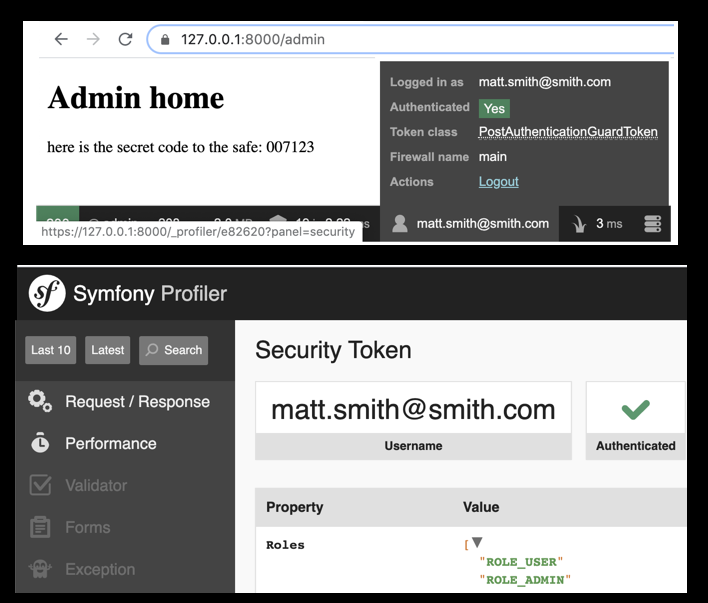
\includegraphics{./tex2pdf.-40a8cafc9587c9a0/63b5ae9f82867fc51df48c24966ee9fcfd7c738c.png}
\caption{Symfony profiler showing ROLE\_USER and ROLE\_ADMIN
authentication. \label{security01}}
\end{figure}

\hypertarget{using-the-logout-route}{%
\section{\texorpdfstring{Using the \texttt{/logout}
route}{Using the /logout route}}\label{using-the-logout-route}}

A logout route \texttt{/logout} was automatically added when we used the
\texttt{make:auth} tool. So we can now use this route to logout the
current user in several ways:

\begin{enumerate}
\def\labelenumi{\arabic{enumi}.}
\item
  We can enter the route directly in the browser address bar, e.g.~via
  URL:

\begin{verbatim}
    http://localhost:8000/logout
\end{verbatim}
\item
  We can also logout via the Symfony profile toolbar. See Figure
  \ref{logout_link}.
\end{enumerate}

\begin{figure}
\centering
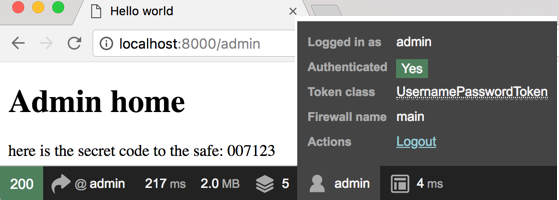
\includegraphics[width=0.75\textwidth,height=\textheight]{./tex2pdf.-40a8cafc9587c9a0/e0059108995273ffa1150aad93ab2af90f546186.png}
\caption{Symfony profiler user logout action. \label{logout_link}}
\end{figure}

In either case we'll logout any currently logged-in user, and return the
anonymously authenticated user \texttt{anon} with no defined
authentication roles.

\hypertarget{finding-and-using-the-internal-loginlogout-route-names-in-securitycontroller}{%
\section{\texorpdfstring{Finding and using the internal login/logout
route names in
\texttt{SecurityController}}{Finding and using the internal login/logout route names in SecurityController}}\label{finding-and-using-the-internal-loginlogout-route-names-in-securitycontroller}}

Look inside the generated
\texttt{/src/controller/SecurityController.php} file to see the
annotation route comments for our login/lgout routes:

\begin{Shaded}
\begin{Highlighting}[]
    \StringTok{...}

    \KeywordTok{class}\NormalTok{ SecurityController }\KeywordTok{extends}\NormalTok{ AbstractController}
\NormalTok{    \{}
        \CommentTok{/**}
\CommentTok{         * }\AnnotationTok{@Route("/login",}\CommentTok{ name="app_login")}
\CommentTok{         */}
        \KeywordTok{public} \KeywordTok{function}\NormalTok{ login}\OtherTok{(}\NormalTok{AuthenticationUtils }\KeywordTok{$authenticationUtils}\OtherTok{)}\NormalTok{: Response}
\NormalTok{        \{}
            \StringTok{...}
\NormalTok{        \}}
    
        \CommentTok{/**}
\CommentTok{         * }\AnnotationTok{@Route("/logout",}\CommentTok{ name="app_logout")}
\CommentTok{         */}
        \KeywordTok{public} \KeywordTok{function}\NormalTok{ logout}\OtherTok{()}
\NormalTok{        \{}
            \StringTok{...}
\NormalTok{        \}}
\end{Highlighting}
\end{Shaded}

We can add links for the user to login/logout on any page in a Twig
template, by using the Twig \texttt{url(...)} function and passing it
the internal route name for our logout route \texttt{app\_logout}, e.g.

\begin{verbatim}
    <a href="{{ url('app_logout') }}">
        logout
    </a>
\end{verbatim}

\hypertarget{security-users-from-database}{%
\chapter{Security users from
database}\label{security-users-from-database}}

\hypertarget{improving-userfixtures-with-a-createuser...-method-project-security03}{%
\section{\texorpdfstring{Improving UserFixtures with a
\texttt{createUser(...)} method (project
\texttt{security03})}{Improving UserFixtures with a createUser(...) method (project security03)}}\label{improving-userfixtures-with-a-createuser...-method-project-security03}}

Since making users in our \texttt{UserFixtures} class is very important,
let's add a \textbf{helper} method to make it very clear what the
properties of each new \texttt{User} object will be. See how clear the
following is, if we have an exrta method \texttt{createUser(...)}:

We need a \texttt{load(...)} method, that gets invoked when we are
loading fixtures from the CLI. This method creates objects for the
entities we want in our database, and the saves (persists) them to the
database:

\begin{Shaded}
\begin{Highlighting}[]
    \KeywordTok{public} \KeywordTok{function}\NormalTok{ load}\OtherTok{(}\NormalTok{ObjectManager }\KeywordTok{$manager}\OtherTok{)}
\NormalTok{    \{}
        \CommentTok{// create objects}
        \KeywordTok{$userUser}\NormalTok{ = }\KeywordTok{$this}\NormalTok{->createUser}\OtherTok{(}\StringTok{'user@user.com'}\OtherTok{,} \StringTok{'user'}\OtherTok{);}
        \KeywordTok{$userAdmin}\NormalTok{ = }\KeywordTok{$this}\NormalTok{->createUser}\OtherTok{(}\StringTok{'admin@admin.com'}\OtherTok{,} \StringTok{'admin'}\OtherTok{,} \OtherTok{[}\StringTok{'ROLE_ADMIN'}\OtherTok{]);}
        \KeywordTok{$userMatt}\NormalTok{ = }\KeywordTok{$this}\NormalTok{->createUser}\OtherTok{(}\StringTok{'matt.smith@smith.com'}\OtherTok{,} \StringTok{'smith'}\OtherTok{,} \OtherTok{[}\StringTok{'ROLE_ADMIN'}\OtherTok{,} \StringTok{'ROLE_SUPER_ADMIN'}\OtherTok{]);}

        \CommentTok{// add to DB queue}
        \KeywordTok{$manager}\NormalTok{->persist}\OtherTok{(}\KeywordTok{$userUser}\OtherTok{);}
        \KeywordTok{$manager}\NormalTok{->persist}\OtherTok{(}\KeywordTok{$userAdmin}\OtherTok{);}
        \KeywordTok{$manager}\NormalTok{->persist}\OtherTok{(}\KeywordTok{$userMatt}\OtherTok{);}

        \CommentTok{// send query to DB}
        \KeywordTok{$manager}\NormalTok{->}\FunctionTok{flush}\OtherTok{();}
\NormalTok{    \}}
\end{Highlighting}
\end{Shaded}

Rather than put all the work in the \texttt{load(...)} method, we can
create a helper method to create each new object. Method
\texttt{createUser(...)} creates and returns a reference to a new
\texttt{User} object given some parameters:

\begin{Shaded}
\begin{Highlighting}[]
    \KeywordTok{private} \KeywordTok{function}\NormalTok{ createUser}\OtherTok{(}\KeywordTok{$username}\OtherTok{,} \KeywordTok{$plainPassword}\OtherTok{,} \KeywordTok{$roles}\NormalTok{ = }\OtherTok{[}\StringTok{'ROLE_USER'}\OtherTok{])}\NormalTok{:User}
\NormalTok{    \{}
        \KeywordTok{$user}\NormalTok{ = }\KeywordTok{new}\NormalTok{ User}\OtherTok{();}
        \KeywordTok{$user}\NormalTok{->setUsername}\OtherTok{(}\KeywordTok{$username}\OtherTok{);}
        \KeywordTok{$user}\NormalTok{->setRoles}\OtherTok{(}\KeywordTok{$roles}\OtherTok{);}

        \CommentTok{// password - and encoding}
        \KeywordTok{$encodedPassword}\NormalTok{ = }\KeywordTok{$this}\NormalTok{->passwordEncoder->encodePassword}\OtherTok{(}\KeywordTok{$user}\OtherTok{,} \KeywordTok{$plainPassword}\OtherTok{);}
        \KeywordTok{$user}\NormalTok{->setPassword}\OtherTok{(}\KeywordTok{$encodedPassword}\OtherTok{);}

        \KeywordTok{return} \KeywordTok{$user}\OtherTok{;}
\NormalTok{    \}}
\end{Highlighting}
\end{Shaded}

NOTE: The default role is \texttt{ROLE\_USER} if none is provided.

\hypertarget{loading-the-fixtures}{%
\section{Loading the fixtures}\label{loading-the-fixtures}}

Loading fixtures involves deleting all existing database contents and
then creating the data from the fixture classes - so you'll get a
warning when loading fixtures. At the CLI type:

\begin{Shaded}
\begin{Highlighting}[]
    \ExtensionTok{symfony}\NormalTok{ console doctrine:fixtures:load}
\end{Highlighting}
\end{Shaded}

That's it!

You should now be able to access \texttt{/admin} with either the
\texttt{matt.smith@smith.com/smith} or \texttt{admin@admin.com/admin}
users. You will get an Access Denied exception if you login with
\texttt{user@user.com/user}, since that only has \texttt{ROLE\_USER}
privileges, and \texttt{ROLE\_ADMIN} is required to visit
\texttt{/admin}.

See Figure \ref{denied_exception} to see the default Symfony (dev mode)
Access Denied exception page.

\begin{figure}
\centering
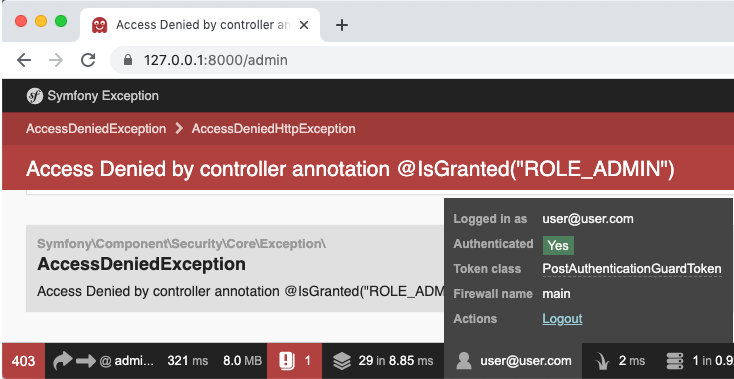
\includegraphics{./tex2pdf.-40a8cafc9587c9a0/f181b091bf6a4a0a60d5cb4a8121508d7ac4b938.png}
\caption{Screenshot of Default Symfony access denied page.
\label{denied_exception}}
\end{figure}

The next chapter will show you how to deal with (and log) access denied
exceptions \ldots{}

\hypertarget{using-sql-from-cli-to-see-users-in-db}{%
\section{Using SQL from CLI to see users in
DB}\label{using-sql-from-cli-to-see-users-in-db}}

To double check your fixtures have been created correctly in the
database, you could run an SQL query from the CLI:

\begin{Shaded}
\begin{Highlighting}[]
\NormalTok{    $ }\ExtensionTok{symfony}\NormalTok{ console doctrine:query:sql }\StringTok{"SELECT * FROM user"}
    \ExtensionTok{Cannot}\NormalTok{ load Xdebug - it was already loaded}
    
    \ExtensionTok{/php-symfony-5-book-codes-security-03-create-user/vendor/doctrine/dbal/lib/Doctrine/DBAL/Tools}\NormalTok{/Dumper.php:}\ExtensionTok{71}\NormalTok{:}
    \ExtensionTok{array}\NormalTok{ (size=3)}
      \ExtensionTok{0}\NormalTok{ =}\OperatorTok{>} 
        \ExtensionTok{array}\NormalTok{ (size=4)}
          \StringTok{'id'}\NormalTok{ =}\OperatorTok{>} \ExtensionTok{string} \StringTok{'2'}\NormalTok{ (length=1)}
          \StringTok{'email'}\NormalTok{ =}\OperatorTok{>} \ExtensionTok{string} \StringTok{'user@user.com'}\NormalTok{ (length=13)}
          \StringTok{'roles'}\NormalTok{ =}\OperatorTok{>} \ExtensionTok{string} \StringTok{'["ROLE_USER"]'}\NormalTok{ (length=13)}
          \StringTok{'password'}\NormalTok{ =}\OperatorTok{>} \ExtensionTok{string} \StringTok{'$2y$13$yfMogZlZfDQ3cJeib6Q2kOqXemYBs.4/AnyK/RbAFp69.360N60ai'}\NormalTok{ (length=60)}
      \ExtensionTok{1}\NormalTok{ =}\OperatorTok{>} 
        \ExtensionTok{array}\NormalTok{ (size=4)}
          \StringTok{'id'}\NormalTok{ =}\OperatorTok{>} \ExtensionTok{string} \StringTok{'3'}\NormalTok{ (length=1)}
          \StringTok{'email'}\NormalTok{ =}\OperatorTok{>} \ExtensionTok{string} \StringTok{'admin@admin.com'}\NormalTok{ (length=15)}
          \StringTok{'roles'}\NormalTok{ =}\OperatorTok{>} \ExtensionTok{string} \StringTok{'["ROLE_ADMIN"]'}\NormalTok{ (length=14)}
          \StringTok{'password'}\NormalTok{ =}\OperatorTok{>} \ExtensionTok{string} \StringTok{'$2y$13$9UyVwrOluOkxLaH57IJM7uPF/NN7iKdBby.z9im2vx4531elfT80a'}\NormalTok{ (length=60)}
      \ExtensionTok{2}\NormalTok{ =}\OperatorTok{>} 
        \ExtensionTok{array}\NormalTok{ (size=4)}
          \StringTok{'id'}\NormalTok{ =}\OperatorTok{>} \ExtensionTok{string} \StringTok{'4'}\NormalTok{ (length=1)}
          \StringTok{'email'}\NormalTok{ =}\OperatorTok{>} \ExtensionTok{string} \StringTok{'matt.smith@smith.com'}\NormalTok{ (length=14)}
          \StringTok{'roles'}\NormalTok{ =}\OperatorTok{>} \ExtensionTok{string} \StringTok{'["ROLE_ADMIN", "ROLE_SUPER_ADMIN"]'}\NormalTok{ (length=34)}
          \StringTok{'password'}\NormalTok{ =}\OperatorTok{>} \ExtensionTok{string} \StringTok{'$2y$13$4/yo6pKgUgECygZHbawemOSeANK78Cu6bGtKKbSgByFLFxASSlC3u'}\NormalTok{ (length=60)}
\end{Highlighting}
\end{Shaded}

\hypertarget{custom-login-page}{%
\chapter{Custom login page}\label{custom-login-page}}

\hypertarget{a-d.i.y.-customisable-login-form-project-security04}{%
\section{\texorpdfstring{A D.I.Y. (customisable) login form (project
\texttt{security04})}{A D.I.Y. (customisable) login form (project security04)}}\label{a-d.i.y.-customisable-login-form-project-security04}}

When we created the Authenticator it created a login form Twig template
for us:

\begin{Shaded}
\begin{Highlighting}[]
\NormalTok{    $ }\ExtensionTok{symfony}\NormalTok{ console make:auth}

    \ExtensionTok{...} 

    \ExtensionTok{created}\NormalTok{: src/Controller/SecurityController.php}
    \ExtensionTok{created}\NormalTok{: templates/security/login.html.twig}
\end{Highlighting}
\end{Shaded}

This is just a Twig template, and we should feel free to look inside and
edit it ourselves \ldots{}

\hypertarget{simplifying-the-generated-login-twig-template}{%
\section{Simplifying the generated login Twig
template}\label{simplifying-the-generated-login-twig-template}}

The generated Twig login page is fine - but you should become confident
in making it your own.

Start by replacing it with this simple, standard HTML login form:

\begin{verbatim}
    <form method="post">
        <h1>Login</h1>

        Username:
        <input value="{{ last_username }}" name="email" id="inputEmail" autofocus>

        <p>
        Password:
        <input type="password" name="password" id="inputPassword">

        <input type="submit" value="Login">

    </form>
\end{verbatim}

The form is shown when the \texttt{/login} URL is visited, or Symfony is
redirected to internal route \texttt{app\_login}, with the HTTP
\texttt{GET} method. There is not \texttt{action} attribute for the
\texttt{\textless{}form\textgreater{}} element, so the form is submitted
to the same router, but using the \texttt{post} method.

Two name/value form variables are submitted:

\begin{itemize}
\item
  \texttt{email} - the email address being used as the unique username
\item
  \texttt{password} - the password
\end{itemize}

\hypertarget{csrf-cross-site-request-forgery-protection}{%
\section{CSRF (Cross Site Request Forgery)
protection}\label{csrf-cross-site-request-forgery-protection}}

Although this Twig template will present a login form to the user, it
will \textbf{not} be accepted by the Symfony security system, due to an
esxposre to CSRF security vulnerability.

NOTE: For any public \textbf{production} site you should always
implement CSRF protection. This is implemented using CSRF `tokens'
created on the server and exchanged with the web client and form
submissions. CSRF tokens help protect web applications against
cross-site scripting request forgery attacks and forged login attacks.

Symfony expects forms to submit a special form variable
\texttt{\_csrf\_token}. In Symfony this token can be generated using
Twig function
\texttt{csrf\_token(\textquotesingle{}authenticate\textquotesingle{})}.
So we need to add this as a hidden form variable for our D.I.Y. form to
work:

\begin{verbatim}
    <form method="post">
        <input type="hidden" name="_csrf_token" value="{{ csrf_token('authenticate') }}">

        ... as before
    </form>
\end{verbatim}

Learn more about CSRF threats and security:

\begin{itemize}
\item
  \href{https://symfony.com/doc/current/security/csrf.html}{Symfony CSRF
  protection}
\item
  \href{https://en.wikipedia.org/wiki/Cross-site_request_forgery\#Forging_login_requests}{Wikipedia}
\item
  \href{https://www.netsparker.com/blog/web-security/protecting-website-using-anti-csrf-token/}{article
  on DIY CSRF for PHP}
\item
  \href{https://stackoverflow.com/questions/6287903/how-to-properly-add-cross-site-request-forgery-csrf-token-using-php}{Stack
  Overlow about PHP CSRF}
\end{itemize}

When using the Symfony generated login form (as we created in this
chapter) the CSRF token protection is built-in automatically.

\hypertarget{display-any-errors}{%
\section{Display any errors}\label{display-any-errors}}

We are only missing one more important set of data from Symfony - any
errors to be displayed due to a previous invalid form submission. We
should always check for an \texttt{error} object, and if present display
its \texttt{messageData} values as follows (here I've added some CSS to
add some padding and a pink background colour):

\begin{verbatim}
    <form method="post">
        <input type="hidden" name="_csrf_token" value="{{ csrf_token('authenticate') }}">

        
            <div style="background-color: pink; padding: 1rem;">
                {{ error.messageKey|trans(error.messageData, 'security') }}
            </div>
        

       <h1>Login</h1>

        Username:
        <input value="{{ last_username }}" name="email" id="inputEmail" autofocus>

        <p>
        Password:
        <input type="password" name="password" id="inputPassword">

        <input type="submit" value="Login">
    </form>
\end{verbatim}

Above we can see the following in our Login Twig template:

\begin{verbatim}
- the HTML `<form>` open tag, which we see submits via HTTP `POST` method

    - no action is given, so the form will submit to the same URL as displayed the form (`/login`), but with a `POST` method

- add the security CSRF token as a hidden form variable    


- display of any Twig `error` variable received

- the `username` label and text input field

    - with 'sticky' form last username value (`last_username`) if any found in the Twig variables

- the `password` label and password input field

- the submit button named `Login`
\end{verbatim}

\hypertarget{custom-login-form-when-attempting-to-access-admin}{%
\section{\texorpdfstring{Custom login form when attempting to access
\texttt{/admin}}{Custom login form when attempting to access /admin}}\label{custom-login-form-when-attempting-to-access-admin}}

See Figure \ref{custom_login_form} to see our custom login form in
action.

\begin{figure}
\centering
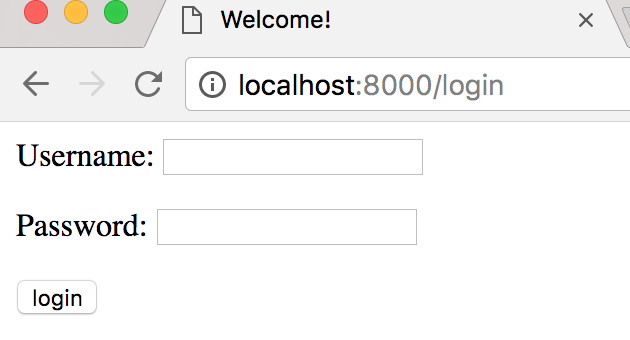
\includegraphics[width=0.75\textwidth,height=\textheight]{./tex2pdf.-40a8cafc9587c9a0/6ae94af6a6d64805890fbeb693bf09927b28b8c9.png}
\caption{Screenshot of custom login form. \label{custom_login_form}}
\end{figure}

\hypertarget{path-for-successful-login}{%
\section{Path for successful login}\label{path-for-successful-login}}

If the user visits the path \texttt{/login} directly in the browser,
Symfony needs to know where to direct the user if login is successful.
This is defined in method \texttt{onAuthenticationSuccess} in class
\texttt{Security/LoginFormAuthenticator}. If no redirect is defined,
then the \texttt{TODO} Exception will be thrown:

\begin{Shaded}
\begin{Highlighting}[]
        \KeywordTok{throw} \KeywordTok{new}\NormalTok{ \textbackslash{}}\KeywordTok{Exception}\OtherTok{(}\StringTok{'TODO: provide a valid redirect inside '}\NormalTok{.}\KeywordTok{__FILE__}\OtherTok{);}
\end{Highlighting}
\end{Shaded}

Since we have a secure \textbf{admin} page, then let's redirect to route
\texttt{admin}:

\begin{Shaded}
\begin{Highlighting}[]
    \KeywordTok{public} \KeywordTok{function}\NormalTok{ onAuthenticationSuccess}\OtherTok{(}\NormalTok{Request }\KeywordTok{$reques§t}\OtherTok{,}\NormalTok{ TokenInterface }\KeywordTok{$token}\OtherTok{,} \KeywordTok{$providerKey}\OtherTok{)}
\NormalTok{    \{}
        \KeywordTok{if} \OtherTok{(}\KeywordTok{$targetPath}\NormalTok{ = }\KeywordTok{$this}\NormalTok{->getTargetPath}\OtherTok{(}\KeywordTok{$request}\NormalTok{->getSession}\OtherTok{(),} \KeywordTok{$providerKey}\OtherTok{))}\NormalTok{ \{}
            \KeywordTok{return} \KeywordTok{new}\NormalTok{ RedirectResponse}\OtherTok{(}\KeywordTok{$targetPath}\OtherTok{);}
\NormalTok{        \}}

        \KeywordTok{return} \KeywordTok{new}\NormalTok{ RedirectResponse}\OtherTok{(}\KeywordTok{$this}\NormalTok{->urlGenerator->generate}\OtherTok{(}\StringTok{'admin'}\OtherTok{));}
\NormalTok{    \}}
\end{Highlighting}
\end{Shaded}

If you want to redirect to different pages, depending on the
\textbf{role} of the newly logged-in user, then do the following:

\begin{itemize}
\item
  get the array of string roles from \texttt{\$token} with
  \texttt{\$token-\textgreater{}getRoles()}
\item
  add \texttt{IF}-statement(s) returning a different named route
  depending on their role, e.g.~something like:

\begin{Shaded}
\begin{Highlighting}[]
    \KeywordTok{if}\OtherTok{(}\FunctionTok{in_array}\OtherTok{(}\StringTok{'ROLE_ADMIN'}\OtherTok{,} \KeywordTok{$roles}\OtherTok{)}\NormalTok{\{        }
        \KeywordTok{return} \KeywordTok{new}\NormalTok{ RedirectResponse}\OtherTok{(}\KeywordTok{$this}\NormalTok{->urlGenerator->generate}\OtherTok{(}\StringTok{'index_admin'}\OtherTok{));}
\NormalTok{    \}        }

    \CommentTok{// else direct to basic staff homne page - or whatever ...}
    \KeywordTok{return} \KeywordTok{new}\NormalTok{ RedirectResponse}\OtherTok{(}\KeywordTok{$this}\NormalTok{->urlGenerator->generate}\OtherTok{(}\StringTok{'index_staff'}\OtherTok{));}
\end{Highlighting}
\end{Shaded}
\end{itemize}

\hypertarget{custom-accessdeniedexception-handler}{%
\chapter{Custom AccessDeniedException
handler}\label{custom-accessdeniedexception-handler}}

\hypertarget{symfony-documentation-for-403-access-denied-exception}{%
\section{Symfony documentation for 403 access denied
exception}\label{symfony-documentation-for-403-access-denied-exception}}

For details about this topic visit the Symfony documentation:

\begin{itemize}
\tightlist
\item
  \url{https://symfony.com/doc/current/security/access_denied_handler.html}
\end{itemize}

\hypertarget{declaring-our-handler-project-security05}{%
\section{\texorpdfstring{Declaring our handler (project
\texttt{security05})}{Declaring our handler (project security05)}}\label{declaring-our-handler-project-security05}}

In \texttt{/config/packages/security.yml} we need to declare that the
class we'll write below will handle access denied exceptions.

So we add this line to the end of our \texttt{main} firewall in
\texttt{security.yml}:

\begin{Shaded}
\begin{Highlighting}[]
    \FunctionTok{access_denied_handler:}\AttributeTok{ App\textbackslash{}Security\textbackslash{}AccessDeniedHandler}
\end{Highlighting}
\end{Shaded}

So the full listing for our \texttt{security.yml} is now:

\begin{Shaded}
\begin{Highlighting}[]
\FunctionTok{security:}
    \FunctionTok{encoders:}
        \FunctionTok{App\textbackslash{}Entity\textbackslash{}User:}
            \FunctionTok{algorithm:}\AttributeTok{ bcrypt}

    \FunctionTok{providers:}
        \FunctionTok{our_db_provider:}
            \FunctionTok{entity:}
                \FunctionTok{class:}\AttributeTok{ App\textbackslash{}Entity\textbackslash{}User}
                \FunctionTok{property:}\AttributeTok{ username}

    \FunctionTok{firewalls:}
        \FunctionTok{dev:}
            \FunctionTok{pattern:}\AttributeTok{ ^/(_(profiler|wdt)|css|images|js)/}
            \FunctionTok{security:}\AttributeTok{ }\CharTok{false}
        \FunctionTok{main:}
            \FunctionTok{anonymous:}\AttributeTok{ }\CharTok{true}
            \FunctionTok{provider:}\AttributeTok{ our_db_provider}
            \FunctionTok{form_login:}
                \FunctionTok{login_path:}\AttributeTok{ login}
                \FunctionTok{check_path:}\AttributeTok{ login}
            \FunctionTok{logout:}
                \FunctionTok{path:}\AttributeTok{   /logout}
                \FunctionTok{target:}\AttributeTok{ /}
            \FunctionTok{access_denied_handler:}\AttributeTok{ App\textbackslash{}Security\textbackslash{}AccessDeniedHandler}
\end{Highlighting}
\end{Shaded}

\hypertarget{the-exception-handler-class}{%
\section{The exception handler
class}\label{the-exception-handler-class}}

Now we needs to write our exception handler class in
\texttt{/src/Security}.

Create new class \texttt{AccessDeniedHandler} in file
\texttt{/src/Security/AccessDeniedHandler.php}:

\begin{Shaded}
\begin{Highlighting}[]
    \KeywordTok{namespace}\NormalTok{ App\textbackslash{}Security}\OtherTok{;}

    \KeywordTok{use}\NormalTok{ Symfony\textbackslash{}Component\textbackslash{}HttpFoundation\textbackslash{}Request}\OtherTok{;}
    \KeywordTok{use}\NormalTok{ Symfony\textbackslash{}Component\textbackslash{}HttpFoundation\textbackslash{}Response}\OtherTok{;}
    \KeywordTok{use}\NormalTok{ Symfony\textbackslash{}Component\textbackslash{}Security\textbackslash{}Core\textbackslash{}}\KeywordTok{Exception}\NormalTok{\textbackslash{}AccessDeniedException}\OtherTok{;}
    \KeywordTok{use}\NormalTok{ Symfony\textbackslash{}Component\textbackslash{}Security\textbackslash{}Http\textbackslash{}Authorization\textbackslash{}AccessDeniedHandlerInterface}\OtherTok{;}

    \KeywordTok{class}\NormalTok{ AccessDeniedHandler }\KeywordTok{implements}\NormalTok{ AccessDeniedHandlerInterface}
\NormalTok{    \{}
        \KeywordTok{public} \KeywordTok{function}\NormalTok{ handle}\OtherTok{(}\NormalTok{Request }\KeywordTok{$request}\OtherTok{,}\NormalTok{ AccessDeniedException }\KeywordTok{$accessDeniedException}\OtherTok{)}
\NormalTok{        \{}
            \KeywordTok{return} \KeywordTok{new}\NormalTok{ Response}\OtherTok{(}\StringTok{'sorry - you have been denied access'}\OtherTok{,} \DecValTok{403}\OtherTok{);}
\NormalTok{        \}}
\NormalTok{    \}}
\end{Highlighting}
\end{Shaded}

That's it!

Now if you try to access \texttt{/admin} with \texttt{user/user} you'll
see the message `sorry - you have been denied access' on screen. See
Figure \ref{denied_exception}.

\begin{figure}
\centering
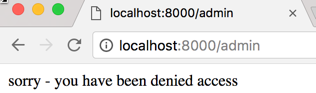
\includegraphics[width=0.75\textwidth,height=\textheight]{./tex2pdf.-40a8cafc9587c9a0/f4cc4aaf3249bfde725a7e233578eed13886be41.png}
\caption{Screenshot of Custom Twig access denied page.
\label{denied_exception}}
\end{figure}

Although it won't be generated through the Twig templating system -
we'll learn how to do that next \ldots{}

\hypertarget{twig-and-logging}{%
\chapter{Twig and logging}\label{twig-and-logging}}

\hypertarget{getting-reference-to-twig-and-logger-objects}{%
\section{Getting reference to Twig and Logger
objects}\label{getting-reference-to-twig-and-logger-objects}}

There are many useful service objects available in the Symfony system
via the `Service Container'. This is a design pattern known as
\textbf{Dependency Injection}. In Symfony we get access to a servce
object by \textbf{Type Hinting} with the server or interface class name,
in the parameter parentheses of the method or constructor of the class.

In this chapter we'll use this technique to get a reference to the Twig
and Logger service objects.

Learn more in the Symfony documentation:

\begin{itemize}
\item
  \url{https://symfony.com/doc/current/service_container.html}
\item
  \url{https://symfony.com/doc/current/components/dependency_injection.html}
\end{itemize}

\hypertarget{using-twig-for-access-denied-message-project-security06}{%
\section{\texorpdfstring{Using Twig for access denied message (project
\texttt{security06})}{Using Twig for access denied message (project security06)}}\label{using-twig-for-access-denied-message-project-security06}}

Let's improved our Access Denied exception handler in 2 ways:

\begin{itemize}
\item
  display a nice Twig template
\item
  log the exception using the standard Monolog logging system
\end{itemize}

First add Monolog to our project with Composer:

\begin{Shaded}
\begin{Highlighting}[]
\NormalTok{    $ }\ExtensionTok{composer}\NormalTok{ req logger}
\end{Highlighting}
\end{Shaded}

Now we will refactor class \texttt{AccessDeniedHandler} to

\begin{Shaded}
\begin{Highlighting}[]
    \KeywordTok{namespace}\NormalTok{ App\textbackslash{}Security}\OtherTok{;}

    \KeywordTok{use}\NormalTok{ Psr\textbackslash{}}\FunctionTok{Log}\NormalTok{\textbackslash{}LoggerInterface}\OtherTok{;}
    \KeywordTok{use}\NormalTok{ Symfony\textbackslash{}Component\textbackslash{}DependencyInjection\textbackslash{}ContainerInterface}\OtherTok{;}
    \KeywordTok{use}\NormalTok{ Symfony\textbackslash{}Component\textbackslash{}HttpFoundation\textbackslash{}Request}\OtherTok{;}
    \KeywordTok{use}\NormalTok{ Symfony\textbackslash{}Component\textbackslash{}HttpFoundation\textbackslash{}Response}\OtherTok{;}
    \KeywordTok{use}\NormalTok{ Symfony\textbackslash{}Component\textbackslash{}Security\textbackslash{}Core\textbackslash{}}\KeywordTok{Exception}\NormalTok{\textbackslash{}AccessDeniedException}\OtherTok{;}
    \KeywordTok{use}\NormalTok{ Symfony\textbackslash{}Component\textbackslash{}Security\textbackslash{}Http\textbackslash{}Authorization\textbackslash{}AccessDeniedHandlerInterface}\OtherTok{;}

    \KeywordTok{class}\NormalTok{ AccessDeniedHandler }\KeywordTok{implements}\NormalTok{ AccessDeniedHandlerInterface}
\NormalTok{    \{}
        \KeywordTok{private} \KeywordTok{$twig}\OtherTok{;}
        \KeywordTok{private} \KeywordTok{$logger}\OtherTok{;}

        \KeywordTok{public} \KeywordTok{function} \FunctionTok{__construct}\OtherTok{(}\NormalTok{ContainerInterface }\KeywordTok{$container}\OtherTok{,}\NormalTok{ LoggerInterface }\KeywordTok{$logger}\OtherTok{)}
\NormalTok{        \{}
            \KeywordTok{$this}\NormalTok{->twig = }\KeywordTok{$container}\NormalTok{->get}\OtherTok{(}\StringTok{'twig'}\OtherTok{);}
            \KeywordTok{$this}\NormalTok{->logger = }\KeywordTok{$logger}\OtherTok{;}
\NormalTok{        \}}

\NormalTok{    \}}
\end{Highlighting}
\end{Shaded}

Now we can re-write method \texttt{handle(...)} to log an error message,
and

\begin{Shaded}
\begin{Highlighting}[]
    \KeywordTok{public} \KeywordTok{function}\NormalTok{ handle}\OtherTok{(}\NormalTok{Request }\KeywordTok{$request}\OtherTok{,}\NormalTok{ AccessDeniedException }\KeywordTok{$accessDeniedException}\OtherTok{)}
\NormalTok{    \{}
        \KeywordTok{$this}\NormalTok{->logger->error}\OtherTok{(}\StringTok{'access denied exception'}\OtherTok{);}

        \KeywordTok{$template}\NormalTok{ = }\StringTok{'error/accessDenied.html.twig'}\OtherTok{;}
        \KeywordTok{$args}\NormalTok{ = }\OtherTok{[];}
        \KeywordTok{$html}\NormalTok{ = }\KeywordTok{$this}\NormalTok{->twig->render}\OtherTok{(}\KeywordTok{$template}\OtherTok{,} \KeywordTok{$args}\OtherTok{);}
        \KeywordTok{return} \KeywordTok{new}\NormalTok{ Response}\OtherTok{(}\KeywordTok{$html}\OtherTok{);}
\NormalTok{    \}}
\end{Highlighting}
\end{Shaded}

\hypertarget{the-twig-page}{%
\section{The Twig page}\label{the-twig-page}}

Create a new folder \texttt{error} in our \texttt{/templates} folder,
and in that create new Twig template \texttt{accessDenied.html.twig} for
our nicer looking error page:

\begin{verbatim}
    
    
    error
    
    
        sorry - access is denied for your request
        <p>
            <a href="{{ url('homepage') }}">home</a>
        </p>
    
\end{verbatim}

Now, login in as \texttt{user@user.com} and try to visit
\texttt{/admin}. We should get that access denied exception again, since
this user does not have the required \texttt{ROLE\_ADMIN} role
privilege. See Figure \ref{denied_log} to see the error log register in
the Symfony profiler footer, at the bottom of our custom error page.

\begin{figure}
\centering
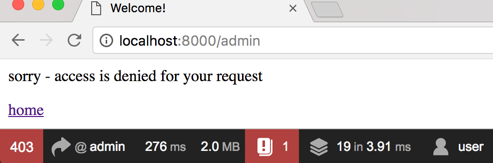
\includegraphics[width=0.75\textwidth,height=\textheight]{./tex2pdf.-40a8cafc9587c9a0/5d7967da5faff673e42573d187ad5b911c5112c2.png}
\caption{Screenshot of Custom Twig access denied page.
\label{denied_log}}
\end{figure}

If you click on the red error you'll see details of all logged messages
during the processing of this request. See Figure \ref{profiler_log}.

\begin{figure}
\centering
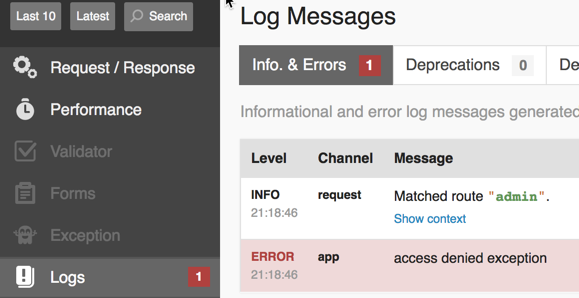
\includegraphics[width=0.75\textwidth,height=\textheight]{./tex2pdf.-40a8cafc9587c9a0/df4541901cd35983e7beb2048b210fa5f1087755.png}
\caption{Screenshot of Profiler log entries. \label{profiler_log}}
\end{figure}

\hypertarget{terminal-log}{%
\section{Terminal log}\label{terminal-log}}

You'll also see a red highlighted error appear in the terminal window if
you are serving this website project with the Symfony web server:

\begin{Shaded}
\begin{Highlighting}[]
\NormalTok{ [}\ExtensionTok{OK}\NormalTok{] Web server listening on https://127.0.0.1:8000 (PHP FPM 7.3.8)                                                    }

    \ExtensionTok{Mar}\NormalTok{ 10 17:11:55 }\KeywordTok{|}\ExtensionTok{WARN} \KeywordTok{|} \ExtensionTok{SERVER}\NormalTok{ GET  (403) }\ExtensionTok{/admin}\NormalTok{ ip=}\StringTok{"127.0.0.1"}
    \ExtensionTok{Mar}\NormalTok{ 10 18:11:54 }\KeywordTok{|}\ExtensionTok{INFO} \KeywordTok{|} \ExtensionTok{REQUES}\NormalTok{ Matched route }\StringTok{"admin"}\NormalTok{. method=}\StringTok{"GET"}\NormalTok{ request_uri=}\StringTok{"https://127.0.0.1:8000/admin"}\NormalTok{ route=}\StringTok{"admin"}\NormalTok{ route_parameters=}\DataTypeTok{\{"_controller":"App\textbackslash{}\textbackslash{}Controller\textbackslash{}\textbackslash{}AdminController::index","_route":"admin"\}}
    \ExtensionTok{Mar}\NormalTok{ 10 18:11:55 }\KeywordTok{|}\ExtensionTok{DEBUG}\KeywordTok{|} \ExtensionTok{SECURI}\NormalTok{ Checking for guard authentication credentials. authenticators=1 firewall_key=}\StringTok{"main"}
        \ExtensionTok{...}\NormalTok{ a bunch more DEBUG logs ....}
    \ExtensionTok{Mar}\NormalTok{ 10 18:11:55 }\KeywordTok{|}\ExtensionTok{DEBUG}\KeywordTok{|} \ExtensionTok{SECURI}\NormalTok{ Access denied, the user is neither anonymous, nor remember-me. }

    \ExtensionTok{Mar}\NormalTok{ 10 18:11:55 }\KeywordTok{|}\ExtensionTok{ERROR}\KeywordTok{|} \ExtensionTok{APP}\NormalTok{    access denied exception  }\OperatorTok{<<<<<<}\NormalTok{ here is our acess denied logged error in the terminal }
\end{Highlighting}
\end{Shaded}

\hypertarget{learn-more-about-logger-and-exceptions}{%
\section{Learn more about logger and
exceptions}\label{learn-more-about-logger-and-exceptions}}

Learn more about Symfony and the Monolog logger:

\begin{itemize}
\tightlist
\item
  \href{http://symfony.com/doc/current/logging.html}{Logging with
  Monolog}
\end{itemize}

Learn more about custom exception handlers and error pages:

\begin{itemize}
\tightlist
\item
  \href{https://symfony.com/doc/current/security/access_denied_handler.html}{Access
  Denied Handler}
\item
  \href{https://symfony.com/doc/current/controller/error_pages.html}{Custom
  Error pages}
\end{itemize}

\hypertarget{user-roles-and-role-hierarchies}{%
\chapter{User roles and role
hierarchies}\label{user-roles-and-role-hierarchies}}

\hypertarget{simplifying-roles-with-a-hierarchy-project-security07}{%
\section{\texorpdfstring{Simplifying roles with a hierarchy (project
\texttt{security07})}{Simplifying roles with a hierarchy (project security07)}}\label{simplifying-roles-with-a-hierarchy-project-security07}}

Let's avoid repeating roles in our program logic (e.g.~IF
\texttt{ROLE\_USER} OR \texttt{ROLE\_ADMIN}) by creating a hierarchy, so
we can give \texttt{ROLE\_ADMIN} all properties of \texttt{ROLE\_USER}
as well. We can easily create a role hierarchy in
\texttt{/config/packages/security.yml}:

\begin{Shaded}
\begin{Highlighting}[]
    \FunctionTok{security:}
        \FunctionTok{role_hierarchy:}
            \FunctionTok{ROLE_ADMIN:}\AttributeTok{       ROLE_USER}

\NormalTok{        ... rest of }\StringTok{'security.yml'}\NormalTok{ as before ...}
\end{Highlighting}
\end{Shaded}

In fact let's go one further - let's create a 3rd user role
(\texttt{ROLE\_SUPER\_ADMIN}) and define that as having all
\texttt{ROLE\_ADMIN} privileges plus the \texttt{ROLE\_USER} privileges
that were inherited by \texttt{ROLE\_ADMIN}:

\begin{Shaded}
\begin{Highlighting}[]
    \FunctionTok{security:}
        \FunctionTok{role_hierarchy:}
            \FunctionTok{ROLE_ADMIN:}\AttributeTok{       ROLE_USER}
            \FunctionTok{ROLE_SUPER_ADMIN:}\AttributeTok{ ROLE_ADMIN}

\NormalTok{        ... rest of }\StringTok{'security.yml'}\NormalTok{ as before ...}
\end{Highlighting}
\end{Shaded}

Now if we log in as a user with \texttt{ROLE\_SUPER\_ADMIN} we also get
\texttt{ROLE\_ADMIN} and \texttt{ROLE\_USER} too!

\hypertarget{modify-fixtures}{%
\section{Modify fixtures}\label{modify-fixtures}}

Now we can modify our fixtures to make user \texttt{matt} have just
\texttt{ROLE\_SUPER\_ADMIN} - the other roles should be inherited
through the hierarchy:

Change \texttt{/src/DataFixtures/UserFixtures.php} as follows:

\begin{Shaded}
\begin{Highlighting}[]
        \KeywordTok{public} \KeywordTok{function}\NormalTok{ load}\OtherTok{(}\NormalTok{ObjectManager }\KeywordTok{$manager}\OtherTok{)}
\NormalTok{        \{}
            \StringTok{...}

            \KeywordTok{$userMatt}\NormalTok{ = }\KeywordTok{$this}\NormalTok{->createUser}\OtherTok{(}\StringTok{'matt.smith@smith.com'}\OtherTok{,} \StringTok{'smith'}\OtherTok{,} \OtherTok{[}\StringTok{'ROLE_SUPER_ADMIN'}\OtherTok{]);}

            \StringTok{...}
\end{Highlighting}
\end{Shaded}

\hypertarget{removing-default-adding-of-role_user-if-using-a-hierarchy}{%
\section{\texorpdfstring{Removing default adding of \texttt{ROLE\_USER}
if using a
hierarchy}{Removing default adding of ROLE\_USER if using a hierarchy}}\label{removing-default-adding-of-role_user-if-using-a-hierarchy}}

If we are using a hierarchy, we don't need always add
\texttt{ROLE\_USER} in code, so we can simplify our getter in our
\texttt{User} Entity in \texttt{/src/Entity/User.php}:

\begin{verbatim}
```php
    public function getRoles()
    {
        return $this->roles;
    }
```
\end{verbatim}

We'll still see \texttt{ROLE\_USER} for admin and super users, but in
the list of \textbf{inherited} roles from the hierarchy. This is show in
Figure \ref{role_inherited}.

\begin{figure}
\centering
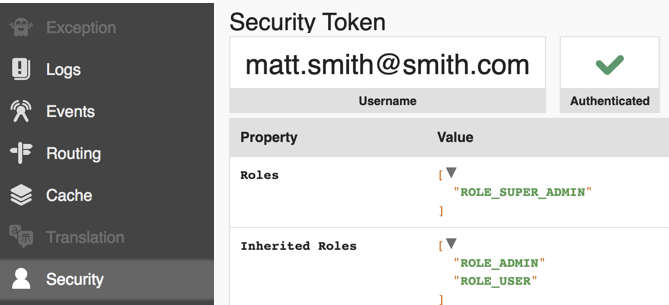
\includegraphics{./tex2pdf.-40a8cafc9587c9a0/2404dfd6a394c9f1aedb6443b74ebf498abf0705.png}
\caption{Super admin user inheriting \texttt{ROLE\_USER}.
\label{role_inherited}}
\end{figure}

Learn about user role hierarchies at:

\begin{itemize}
\tightlist
\item
  \href{https://symfony.com/doc/current/security.html\#hierarchical-roles}{Symfony
  hierarchical roles}
\end{itemize}

\hypertarget{allowing-easy-switching-of-users-when-debugging}{%
\section{Allowing easy switching of users when
debugging}\label{allowing-easy-switching-of-users-when-debugging}}

If you wish to speed up testing, you can allow easy switching between
users just by adding a but at the end of your request URL, \textbf{if}
you add the following to your firewall:

\begin{Shaded}
\begin{Highlighting}[]
    \FunctionTok{switch_user:}\AttributeTok{ }\CharTok{true}
\end{Highlighting}
\end{Shaded}

Now you can switch users bu adding the following at the end of the URL:

\begin{verbatim}
    ?_switch_user=<username>
\end{verbatim}

You stop impersonating users by adding \texttt{?\_switch\_user=\_exit}
to the end of a URL.

For example to visit the home page as user \texttt{user} you would write
this URL:

\begin{verbatim}
    http://localhost:8000/?_switch_user=user
\end{verbatim}

In your Twig you can allow this user to see special content (e.g.~a link
to exit impersonation) by testing for the special (automatically created
role) \texttt{ROLE\_PREVIOUS\_ADMIN}:

\begin{verbatim}
    
        <a href="{{ path('admin_index', {'_switch_user': '_exit'}) }}">Exit impersonation & return to admin home</a>
    
\end{verbatim}

Learn more at:

\begin{itemize}
\tightlist
\item
  \href{https://symfony.com/doc/current/security/impersonating_user.html}{Impersonating
  users}
\end{itemize}

\hypertarget{customising-view-based-on-logged-in-user}{%
\chapter{Customising view based on logged-in
user}\label{customising-view-based-on-logged-in-user}}

\hypertarget{twig-nav-links-when-logged-in-project-security08}{%
\section{\texorpdfstring{Twig nav links when logged in (project
\texttt{security08})}{Twig nav links when logged in (project security08)}}\label{twig-nav-links-when-logged-in-project-security08}}

The
\href{https://symfony.com/doc/current/security.html\#fetch-the-user-in-a-template}{Symfony
security docs} give us the Twig code for a conditional statement for
when the current user has logged in:

\begin{Shaded}
\begin{Highlighting}[]
\NormalTok{    \{% if is_granted('IS_AUTHENTICATED_FULLY') %\}}
        \KeywordTok{<p>}\NormalTok{Username: \{\{ app.user.username \}\}}\KeywordTok{</p>}
\NormalTok{    \{% endif %\}}
\end{Highlighting}
\end{Shaded}

We can also test for which \textbf{role} a user may have granted when
logged-in, e.g.:

\begin{Shaded}
\begin{Highlighting}[]
\NormalTok{    \{% if is_granted('ROLE_ADMIN') %\}}
\NormalTok{          Welcome to the Admin home page ...}
\NormalTok{    \{% endif %\}}
\end{Highlighting}
\end{Shaded}

We can use such conditionals in 2 useful and common ways:

\begin{enumerate}
\def\labelenumi{\arabic{enumi}.}
\item
  Confirm the login username and offer a \texttt{logout} link for users
  who are logged in
\item
  Have navbar links revealed only for logged-in users (of particular
  roles)
\end{enumerate}

So let's add such code to our \texttt{base.html.twig} master template
(in \texttt{/templates}).

First, let's add a \texttt{\textless{}header\textgreater{}} element to
either show the username and a logout link, or a link to login if the
user is not logged-in yet:

\begin{verbatim}
    <header>
        
            Username:
            <strong>{{ app.user.username }}</strong>
            <br>
            <a href="{{ url('app_logout') }}">logout</a>
        
            <a href="{{ url('app_login') }}">login</a>
        
    </header>
\end{verbatim}

We can right align it and have a black bottom border with a little style
in the \texttt{\textless{}head\textgreater{}}:

\begin{Shaded}
\begin{Highlighting}[]
\NormalTok{    <!DOCTYPE html}\OperatorTok{>}
\NormalTok{    <html}\OperatorTok{>}
\NormalTok{        <head}\OperatorTok{>}
\NormalTok{            <meta charset="UTF-8"}\OperatorTok{>}
\NormalTok{            <title}\OperatorTok{>}\NormalTok{\{% block title %\}Welcome!\{% endblock %\}</title}\OperatorTok{>}

\NormalTok{            <style}\OperatorTok{>}
\NormalTok{                header \{}
                    \KeywordTok{text-align}\NormalTok{: }\DecValTok{right}\OperatorTok{;}
                    \KeywordTok{border-bottom}\NormalTok{: }\DecValTok{0.5}\DataTypeTok{rem} \DecValTok{solid} \ConstantTok{black}\OperatorTok{;}
                    \KeywordTok{padding}\NormalTok{: }\DecValTok{1}\DataTypeTok{rem}\OperatorTok{;}
\NormalTok{                \}}
\NormalTok{            </style}\OperatorTok{>}
\end{Highlighting}
\end{Shaded}

Next, let's define a \texttt{\textless{}nav\textgreater{}} element, so
that \textbf{all} users see a link to the homepage on every page on the
website (at least those that extend \texttt{base.html.twig}). We will
also add a conditional navigation link - to that users logged-in with
\texttt{ROLE\_ADMIN} can also see a link to the admin home page:

\begin{verbatim}
    <nav>
        <ul>
            <li>
                <a href="{{ url('homepage') }}">home</a>
            </li>

            
                <li>
                    <a href="{{ url('admin') }}">admin home</a>
                </li>
            
        </ul>
    </nav>
\end{verbatim}

So when a user first visits our website homepage, they are not
logged-in, so will see a \texttt{login} link in the header, and the
navigation bar will only show a link to this homepage. See Figure
\ref{homepage_login_link}.

\begin{figure}
\centering
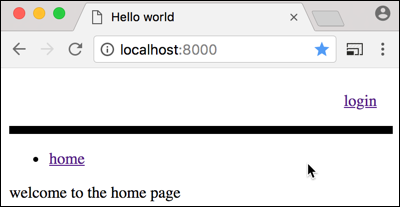
\includegraphics[width=0.6\textwidth,height=\textheight]{./tex2pdf.-40a8cafc9587c9a0/37775f03f58d57201d8d743fdd9e86349205c708.png}
\caption{Screenshot of homepage before logging-in.
\label{homepage_login_link}}
\end{figure}

If the user has successfully logged-in with a \texttt{ROLE\_ADMIN}
privilege account, they will now see their userame and a \texttt{logout}
link in the header, and they will also see revealed a link to the admin
home page. See Figure \ref{admin_user_homepage}.

\begin{figure}
\centering
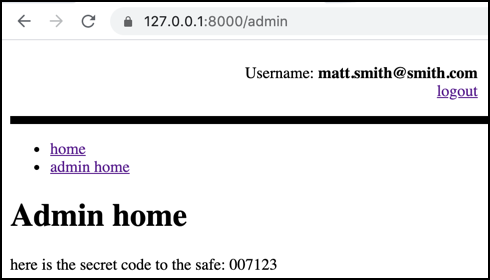
\includegraphics[width=0.6\textwidth,height=\textheight]{./tex2pdf.-40a8cafc9587c9a0/49ec37103f4f81567fa2694c122b38f522d2b6be.png}
\caption{Screenshot of homepage after \texttt{ROLE\_ADMIN} has
logged-in.\label{admin_user_homepage}}
\end{figure}

\hypertarget{getting-reference-to-the-current-user-in-a-controller}{%
\section{Getting reference to the current user in a
Controller}\label{getting-reference-to-the-current-user-in-a-controller}}

in PHP (e.g.~a controller) you can get the user object as follows:

\begin{Shaded}
\begin{Highlighting}[]
    \KeywordTok{$user}\NormalTok{ = }\KeywordTok{$this}\NormalTok{->getUser}\OtherTok{();}
\end{Highlighting}
\end{Shaded}

or you can type-hint in a controller method declaration, and the param
converter will provide the \$security object for your to interrogate:

\begin{Shaded}
\begin{Highlighting}[]
    \KeywordTok{use}\NormalTok{ Symfony\textbackslash{}Component\textbackslash{}Security\textbackslash{}Core\textbackslash{}Security}\OtherTok{;}

    \KeywordTok{public} \KeywordTok{function}\NormalTok{ indexAction}\OtherTok{(}\NormalTok{Security }\KeywordTok{$security}\OtherTok{)}
\NormalTok{    \{}
        \KeywordTok{$user}\NormalTok{ = }\KeywordTok{$security}\NormalTok{->getUser}\OtherTok{();}
\NormalTok{    \}}
\end{Highlighting}
\end{Shaded}

see:

\begin{itemize}
\tightlist
\item
  \url{https://symfony.com/doc/current/security.html\#a-fetching-the-user-object}
\end{itemize}

\hypertarget{simplifying-roles-and-adding-secure-user-crud-project-security09}{%
\chapter{\texorpdfstring{Simplifying roles and adding secure User CRUD
(project
\texttt{security09})}{Simplifying roles and adding secure User CRUD (project security09)}}\label{simplifying-roles-and-adding-secure-user-crud-project-security09}}

\hypertarget{user-crud-problem-1-an-array-of-roles}{%
\section{User CRUD PROBLEM 1: an array of
ROLES}\label{user-crud-problem-1-an-array-of-roles}}

If we try to generate CRUD for our system \texttt{User} we'll hit a
problem when trying to enter a String for the ROLE, since the default
Symfony \texttt{User} stores roles in an array.

Try it:

\begin{itemize}
\tightlist
\item
  generate CRUD for entity \texttt{User}
\item
  try to create a new user
\item
  you'll get an error about string/array mismatch when you enter
  something like \texttt{ROLE\_ADMIN} for the new \texttt{User} role
\end{itemize}

\hypertarget{user-crud-problem-1-a-solution}{%
\section{User CRUD PROBLEM 1: a
solution}\label{user-crud-problem-1-a-solution}}

I find the simplest solution is to use a role hierarchy (see previous
chapter), so we only need to store a single ROLE string for a
\texttt{User}.

However, to meet the requirements for the Symfony security system, the
\texttt{User} class must have a \texttt{getRoles()} method that returns
an array.

The solution is pretty straightforward:

\begin{enumerate}
\def\labelenumi{\arabic{enumi}.}
\item
  add a new String \texttt{role} property to the \texttt{User} entity

  \begin{itemize}
  \tightlist
  \item
    HINT: use \texttt{make:entity\ User} and add the new property
  \end{itemize}
\item
  change the \texttt{getRoles()} method to simply return the string
  \texttt{role} wrapped in an array:

\begin{Shaded}
\begin{Highlighting}[]
\KeywordTok{public} \KeywordTok{function}\NormalTok{ getRoles}\OtherTok{()}\NormalTok{: }\KeywordTok{array}
\NormalTok{\{}
    \KeywordTok{return} \OtherTok{[}\KeywordTok{$this}\NormalTok{->role}\OtherTok{];}
\NormalTok{\}}
\end{Highlighting}
\end{Shaded}
\item
  delete the \texttt{roles} property and the \texttt{setRoles(...)}
  method from entity \texttt{User}
\item
  update your \texttt{UserFixtures} fixtures to set the \texttt{role}
  property - not using arrays \ldots{}
\end{enumerate}

\begin{Shaded}
\begin{Highlighting}[]
    \KeywordTok{public} \KeywordTok{function}\NormalTok{ load}\OtherTok{(}\NormalTok{ObjectManager }\KeywordTok{$manager}\OtherTok{)}
\NormalTok{    \{}
        \CommentTok{// create objects}
        \KeywordTok{$userUser}\NormalTok{ = }\KeywordTok{$this}\NormalTok{->createUser}\OtherTok{(}\StringTok{'user@user.com'}\OtherTok{,} \StringTok{'user'}\OtherTok{);}
        \KeywordTok{$userAdmin}\NormalTok{ = }\KeywordTok{$this}\NormalTok{->createUser}\OtherTok{(}\StringTok{'admin@admin.com'}\OtherTok{,} \StringTok{'admin'}\OtherTok{,} \StringTok{'ROLE_ADMIN'}\OtherTok{);}
        \KeywordTok{$userMatt}\NormalTok{ = }\KeywordTok{$this}\NormalTok{->createUser}\OtherTok{(}\StringTok{'matt.smith@smith.com'}\OtherTok{,} \StringTok{'smith'}\OtherTok{,} \StringTok{'ROLE_SUPER_ADMIN'}\OtherTok{);}

        \CommentTok{// add to DB queue}
        \KeywordTok{$manager}\NormalTok{->persist}\OtherTok{(}\KeywordTok{$userUser}\OtherTok{);}
        \KeywordTok{$manager}\NormalTok{->persist}\OtherTok{(}\KeywordTok{$userAdmin}\OtherTok{);}
        \KeywordTok{$manager}\NormalTok{->persist}\OtherTok{(}\KeywordTok{$userMatt}\OtherTok{);}

        \CommentTok{// send query to DB}
        \KeywordTok{$manager}\NormalTok{->}\FunctionTok{flush}\OtherTok{();}

\NormalTok{    \}}

    \KeywordTok{private} \KeywordTok{function}\NormalTok{ createUser}\OtherTok{(}\KeywordTok{$username}\OtherTok{,} \KeywordTok{$plainPassword}\OtherTok{,} \KeywordTok{$role}\NormalTok{ = }\StringTok{'ROLE_USER'}\OtherTok{)}\NormalTok{:User}
\NormalTok{    \{}
        \KeywordTok{$user}\NormalTok{ = }\KeywordTok{new}\NormalTok{ User}\OtherTok{();}
        \KeywordTok{$user}\NormalTok{->setEmail}\OtherTok{(}\KeywordTok{$username}\OtherTok{);}
        \KeywordTok{$user}\NormalTok{->setRole}\OtherTok{(}\KeywordTok{$role}\OtherTok{);}
\end{Highlighting}
\end{Shaded}

\begin{enumerate}
\def\labelenumi{\arabic{enumi}.}
\item
  migrate the DB
\item
  load the fixtures
\item
  delete the old CRUD and create new CRUD
\end{enumerate}

\hypertarget{user-crud-problem-2-plain-test-password-stored-in-db}{%
\section{User CRUD PROBLEM 2: plain test password stored in
DB}\label{user-crud-problem-2-plain-test-password-stored-in-db}}

The default CRUD generation will store in the DB whatever plain text
password is entered in the form.

But, the Symfony security systems expects a \textbf{hashed} password to
be stored in the DB, so we have 2 problems:

\begin{enumerate}
\def\labelenumi{\arabic{enumi}.}
\item
  we should \textbf{never} store plain text passwords in the DB
\item
  we cannot login, since the security system will think the stored text
  is a bad bash
\end{enumerate}

\hypertarget{user-crud-problem-2-a-solution}{%
\section{User CRUD PROBLEM 2: a
solution}\label{user-crud-problem-2-a-solution}}

We can solve this problem the same way we encoded passwords in our
\texttt{UserFixtures} - by adding a password encoder, and hashing the
plain text password before the object's contents is persisted to the DB.

Do the following to our CRUD controller class \texttt{UserController}:

\begin{enumerate}
\def\labelenumi{\arabic{enumi}.}
\item
  add a \texttt{use} statement for class
  \texttt{UserPasswordEncoderInterface}

\begin{Shaded}
\begin{Highlighting}[]
\KeywordTok{use}\NormalTok{ Symfony\textbackslash{}Component\textbackslash{}Security\textbackslash{}Core\textbackslash{}Encoder\textbackslash{}UserPasswordEncoderInterface}\OtherTok{;}
\end{Highlighting}
\end{Shaded}
\item
  for the \texttt{new} route we need to add a \texttt{\$passwordEncoder}
  to the method arguments (the Symfony param-converter will magically
  create the object for us to use), and then we can encode the plaintext
  password and use the \texttt{setPassword(...)} method to ensure that
  it is the \textbf{hashed} password stored in the DB:

\begin{Shaded}
\begin{Highlighting}[]
\CommentTok{/**}
\CommentTok{ * }\AnnotationTok{@Route("/new",}\CommentTok{ name="user_new", methods=\{"GET","POST"\})}
\CommentTok{ */}
\KeywordTok{public} \KeywordTok{function} \KeywordTok{new}\OtherTok{(}\NormalTok{Request }\KeywordTok{$request}\OtherTok{,}\NormalTok{ UserPasswordEncoderInterface }\KeywordTok{$passwordEncoder}\OtherTok{)}\NormalTok{: Response}
\NormalTok{\{}
    \KeywordTok{$user}\NormalTok{ = }\KeywordTok{new}\NormalTok{ User}\OtherTok{();}
    \KeywordTok{$form}\NormalTok{ = }\KeywordTok{$this}\NormalTok{->createForm}\OtherTok{(}\NormalTok{UserType::}\KeywordTok{class}\OtherTok{,} \KeywordTok{$user}\OtherTok{);}
    \KeywordTok{$form}\NormalTok{->handleRequest}\OtherTok{(}\KeywordTok{$request}\OtherTok{);}

    \KeywordTok{if} \OtherTok{(}\KeywordTok{$form}\NormalTok{->isSubmitted}\OtherTok{()}\NormalTok{ && }\KeywordTok{$form}\NormalTok{->isValid}\OtherTok{())}\NormalTok{ \{}
        \KeywordTok{$entityManager}\NormalTok{ = }\KeywordTok{$this}\NormalTok{->getDoctrine}\OtherTok{()}\NormalTok{->getManager}\OtherTok{();}

        \CommentTok{// encode password}
        \KeywordTok{$plainPassword}\NormalTok{ = }\KeywordTok{$user}\NormalTok{->getPassword}\OtherTok{();}
        \KeywordTok{$encodedPassword}\NormalTok{ = }\KeywordTok{$passwordEncoder}\NormalTok{->encodePassword}\OtherTok{(}\KeywordTok{$user}\OtherTok{,} \KeywordTok{$plainPassword}\OtherTok{);}
        \KeywordTok{$user}\NormalTok{->setPassword}\OtherTok{(}\KeywordTok{$encodedPassword}\OtherTok{);}

        \KeywordTok{$entityManager}\NormalTok{->persist}\OtherTok{(}\KeywordTok{$user}\OtherTok{);}
        \KeywordTok{$entityManager}\NormalTok{->}\FunctionTok{flush}\OtherTok{();}
\end{Highlighting}
\end{Shaded}
\item
  do the same for the \textbf{edit} route:

\begin{Shaded}
\begin{Highlighting}[]
\CommentTok{/**}
\CommentTok{ * }\AnnotationTok{@Route("/\{id\}/edit",}\CommentTok{ name="user_edit", methods=\{"GET","POST"\})}
\CommentTok{ */}
\KeywordTok{public} \KeywordTok{function}\NormalTok{ edit}\OtherTok{(}\NormalTok{Request }\KeywordTok{$request}\OtherTok{,}\NormalTok{ User }\KeywordTok{$user}\OtherTok{,}\NormalTok{ UserPasswordEncoderInterface }\KeywordTok{$passwordEncoder}\OtherTok{)}\NormalTok{: Response}
\NormalTok{\{}
    \KeywordTok{$form}\NormalTok{ = }\KeywordTok{$this}\NormalTok{->createForm}\OtherTok{(}\NormalTok{UserType::}\KeywordTok{class}\OtherTok{,} \KeywordTok{$user}\OtherTok{);}
    \KeywordTok{$form}\NormalTok{->handleRequest}\OtherTok{(}\KeywordTok{$request}\OtherTok{);}

    \KeywordTok{if} \OtherTok{(}\KeywordTok{$form}\NormalTok{->isSubmitted}\OtherTok{()}\NormalTok{ && }\KeywordTok{$form}\NormalTok{->isValid}\OtherTok{())}\NormalTok{ \{}

        \CommentTok{// encode password}
        \KeywordTok{$plainPassword}\NormalTok{ = }\KeywordTok{$user}\NormalTok{->getPassword}\OtherTok{();}
        \KeywordTok{$encodedPassword}\NormalTok{ = }\KeywordTok{$passwordEncoder}\NormalTok{->encodePassword}\OtherTok{(}\KeywordTok{$user}\OtherTok{,} \KeywordTok{$plainPassword}\OtherTok{);}
        \KeywordTok{$user}\NormalTok{->setPassword}\OtherTok{(}\KeywordTok{$encodedPassword}\OtherTok{);}

        \KeywordTok{$this}\NormalTok{->getDoctrine}\OtherTok{()}\NormalTok{->getManager}\OtherTok{()}\NormalTok{->}\FunctionTok{flush}\OtherTok{();}
\end{Highlighting}
\end{Shaded}
\end{enumerate}

See Figure \ref{userCrud} to see new user \texttt{test@test.com} with
correctly stored hashed password.

\begin{figure}
\centering
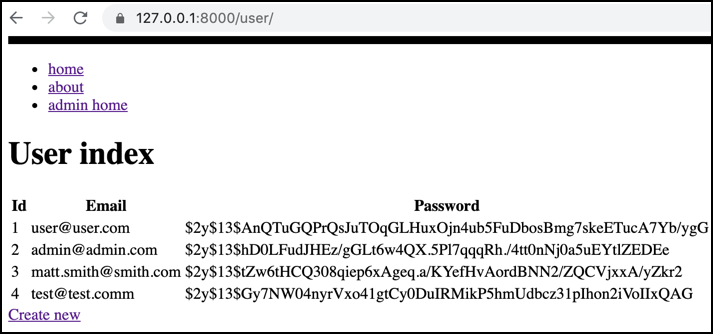
\includegraphics{./tex2pdf.-40a8cafc9587c9a0/8ca93997f444ca616cd3203a26c977fbf5b2792c.png}
\caption{Screenshot of Admin User CRUD with stored hased passwords.
\label{userCrud}}
\end{figure}

\hypertarget{securing-the-user-crud-for-role_admin-only}{%
\section{\texorpdfstring{Securing the \texttt{User} CRUD for
\texttt{ROLE\_ADMIN}
only}{Securing the User CRUD for ROLE\_ADMIN only}}\label{securing-the-user-crud-for-role_admin-only}}

We can secure all routes in our CRUD \texttt{UserController} by:

\begin{itemize}
\item
  adding a \texttt{use} statement for the \texttt{IsGranted} class
\item
  adding an \texttt{@IsGranted} annotation comment immdiately
  \textbf{before} the class delcaration

\begin{Shaded}
\begin{Highlighting}[]
\KeywordTok{<?php}

\KeywordTok{namespace}\NormalTok{ App\textbackslash{}Controller}\OtherTok{;}

\KeywordTok{use}\NormalTok{ App\textbackslash{}Entity\textbackslash{}User}\OtherTok{;}
\KeywordTok{use}\NormalTok{ App\textbackslash{}Form\textbackslash{}UserType}\OtherTok{;}
\KeywordTok{use}\NormalTok{ App\textbackslash{}Repository\textbackslash{}UserRepository}\OtherTok{;}
\KeywordTok{use}\NormalTok{ Symfony\textbackslash{}Bundle\textbackslash{}FrameworkBundle\textbackslash{}Controller\textbackslash{}AbstractController}\OtherTok{;}
\KeywordTok{use}\NormalTok{ Symfony\textbackslash{}Component\textbackslash{}HttpFoundation\textbackslash{}Request}\OtherTok{;}
\KeywordTok{use}\NormalTok{ Symfony\textbackslash{}Component\textbackslash{}HttpFoundation\textbackslash{}Response}\OtherTok{;}
\KeywordTok{use}\NormalTok{ Symfony\textbackslash{}Component\textbackslash{}Routing\textbackslash{}Annotation\textbackslash{}Route}\OtherTok{;}
\KeywordTok{use}\NormalTok{ Symfony\textbackslash{}Component\textbackslash{}Security\textbackslash{}Core\textbackslash{}Encoder\textbackslash{}UserPasswordEncoderInterface}\OtherTok{;}

\KeywordTok{use}\NormalTok{ Sensio\textbackslash{}Bundle\textbackslash{}FrameworkExtraBundle\textbackslash{}Configuration\textbackslash{}IsGranted}\OtherTok{;}


\CommentTok{/**}
\CommentTok{ * }\AnnotationTok{@IsGranted("ROLE_ADMIN")}
\CommentTok{ * }\AnnotationTok{@Route("/user")}
\CommentTok{ */}
\KeywordTok{class}\NormalTok{ UserController }\KeywordTok{extends}\NormalTok{ AbstractController}
\NormalTok{\{}
\end{Highlighting}
\end{Shaded}
\end{itemize}

\hypertarget{further-steps}{%
\section{Further steps}\label{further-steps}}

Rather than typing in text like\texttt{ROLE\_USER} and
\texttt{ROLE\_ADMIN}, it would be nice to choose them from a dropdown
list - via an associated \texttt{Role} entity \ldots{} \backmatter

\hypertarget{list-of-references}{%
\chapter{List of References}\label{list-of-references}}

\end{document}
